\documentclass[uplatex, a4paper, 12pt, openany, oneside]{jsbook}

\usepackage[dvipdfmx]{graphicx}
\usepackage[dvipdfmx]{color}
\usepackage[dvipdfmx, bookmarks=true, setpagesize=false]{hyperref}
\usepackage{pxjahyper}

\usepackage{thesis}
\usepackage{here}
\usepackage{url}
\usepackage{amsmath}
\usepackage{amssymb}
\usepackage{amsfonts}
% \usepackage{CJKutf8}

\thesis{修 士 論 文}
\title{
  \centering
    \scalebox{1.0}{移動ロボットのための深層学習を用いた}
    \vspace{-0.3zh}
    \scalebox{1.0}{歩行者の位置予測とナビゲーションへの応用}
    \vspace{-0.3zh}
    \scalebox{0.6}{Pedestrian Position Prediction Using Deep Learning for Mobile Robots}
    \vspace{-0.6zh}
    \scalebox{0.6}{and Its Application to Navigation}
    \vspace{-0.6zh}
}
\setlength{\textwidth}{\fullwidth}
\setlength{\evensidemargin}{\oddsidemargin}

\date{\today}
\vspace{-15.0zh}
\teacher{林原 靖男 教授}
\vspace{-15.0zh}
\organization{千葉工業大学 先進工学部 未来ロボティクス学科}
\author{23S1030 藤原柾}
\vspace{-15zh}

\renewcommand{\baselinestretch}{1.2}
\begin{document}

%% Front Matter
\frontmatter{}
%
\chapter{実験}
\label{chap:experiments}
この章では, 1節で我々が行ってきた研究\cite{mech}の実験(以下, 「従来の実験」と称する)を実環境に移行する際に, 新たに顕在化した課題点について述べる. また, 課題を解決するための2つのアプローチを提案し, 実験と検証を行う. 2節では, 実験に簡易的なシミュレータを用いる問題点を述べ, 解決策を提示する. 3節では, 実環境で実験を行い, 実環境における提案手法の有効性を検証する.  
%
%\input{experiments/preface}
%
%!TEX root = ../thesis.tex

\section{実験要件}
実験には下記のコンピュータとソフトウェアを用いた. 

\begin{enumerate}
  \item コンピュータ\\
  OS: Ubuntu 20.04 LTS\\
  ROS: Noetic\\
  CPU: intel Core i7-10700F(4.8GHz/8コア/16スレッド)\\
  DRAM: 32GB DDR4(3200/8GB×4)
  \item nav\_cloning(学習器, 統合環境)\\
  \url{https://github.com/open-rdc/nav_cloning}
  \item waypoint\_nav(移動目標地点, 目標方向を出力)\\
  \url{https://github.com/open-rdc/waypoint_nav}
  \newpage
  \item turtlebot3 関連\\
  \url{https://github.com/open-rdc/turtlebot3}
  \item navigation(ナビゲーションパッケージ)\\
  \url{https://github.com/ros-planning/navigation}
\end{enumerate}

\subsection{実験装置(シミュレータ)}

\begin{itemize}
  \item ロボット

ロボットモデルは前報\cite{okada1}\cite{okada2}と同様, \figref{Fig:waffle_pi}に示すように, TurtleBot3 Waffle\_piへ3つのカメラを追加したモデルを用いる.

\begin{figure}[hbtp]
  \centering
 \includegraphics[keepaspectratio, scale=0.22]
      {images/Waffle_pi.png}
 \caption{TurtleBot3 waffle\_pi with 3 cameras}
 \label{Fig:waffle_pi}
\end{figure}

\item 環境\\
シミュレータ環境として, オープンソースの3DロボットシミュレータGazeboを用いる. \figref{Fig:sim}に示すようなGazebo上で千葉工業大学2号館3階を模した実験環境を対象に実験を行う.

\begin{figure}[hbtp]
  \centering
 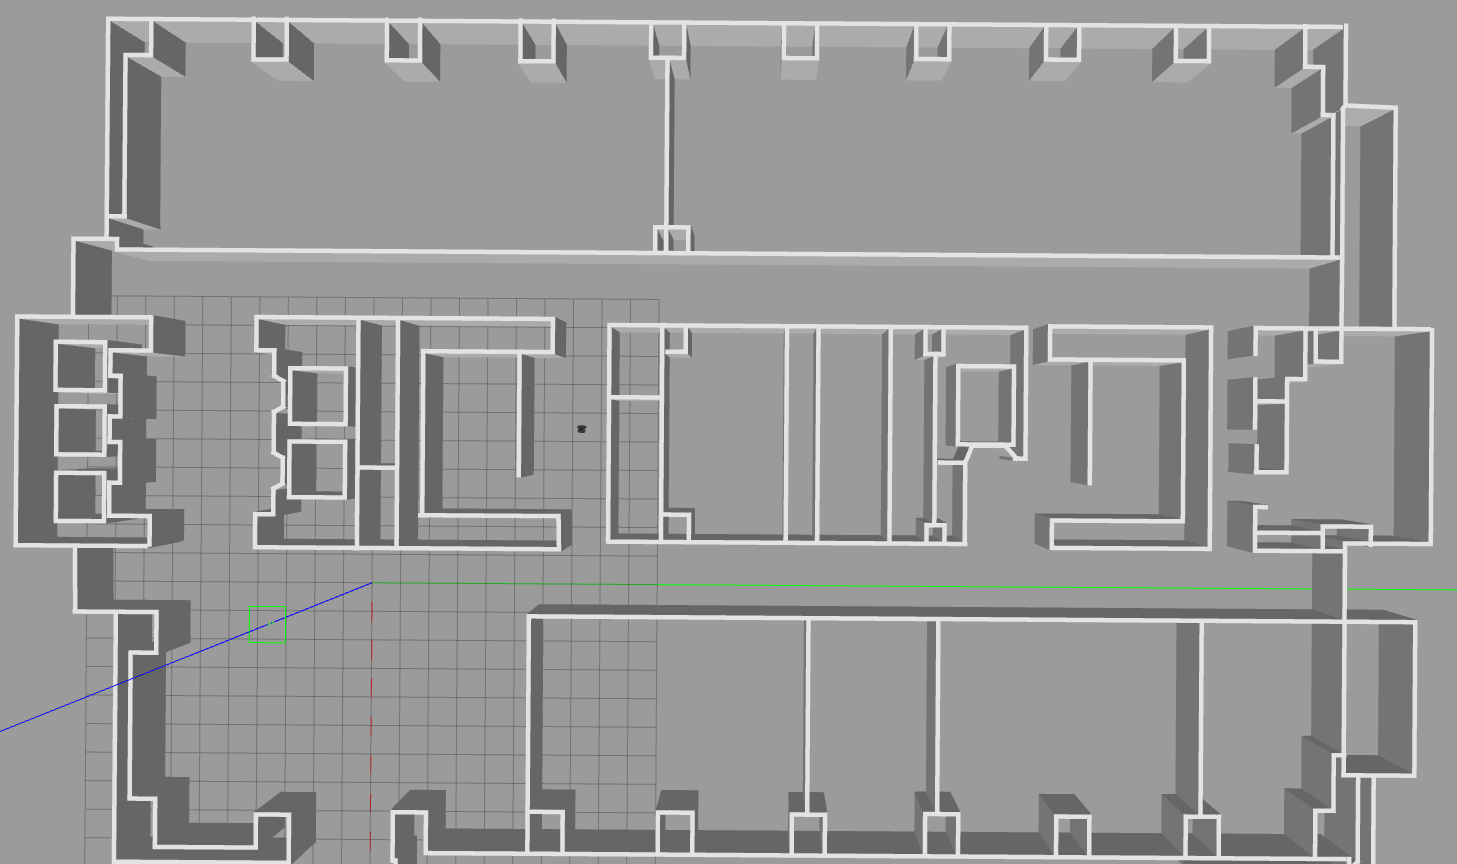
\includegraphics[keepaspectratio, scale=0.12]
      {images/tsudanuma2-3_simorg.png}
 \caption{Experimental enviroment of simulator}
 \label{Fig:sim}
\end{figure}

\end{itemize}

\subsection{実験方法}
\figref{Fig:sim_explain}のA, B地点において, \figref{Fig:select}に示すように侵入する方向が3つあり, 進むことのできる方向が2つあることから, 1箇所につき走行パターンが6つ存在する. 
また, A, B地点では, 目標方向に従って任意の経路を選択することが求められる場所である.
したがって, 実験ではA, B地点で合計12パターンの走行において, 与えた目標方向に従った行動が行えるのかを確認する.

\begin{figure}[hbtp]
  \centering
 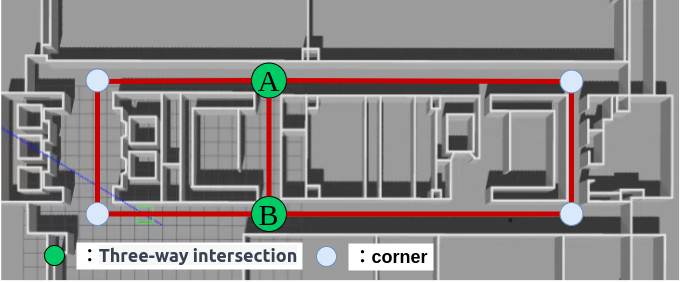
\includegraphics[keepaspectratio, scale=0.5]
      {images/sim_explain.png}
 \caption{Characteristics of passages in the experimental environment on the simulator}
 \label{Fig:sim_explain}
\end{figure}

\begin{figure}[hbtp]
  \centering
 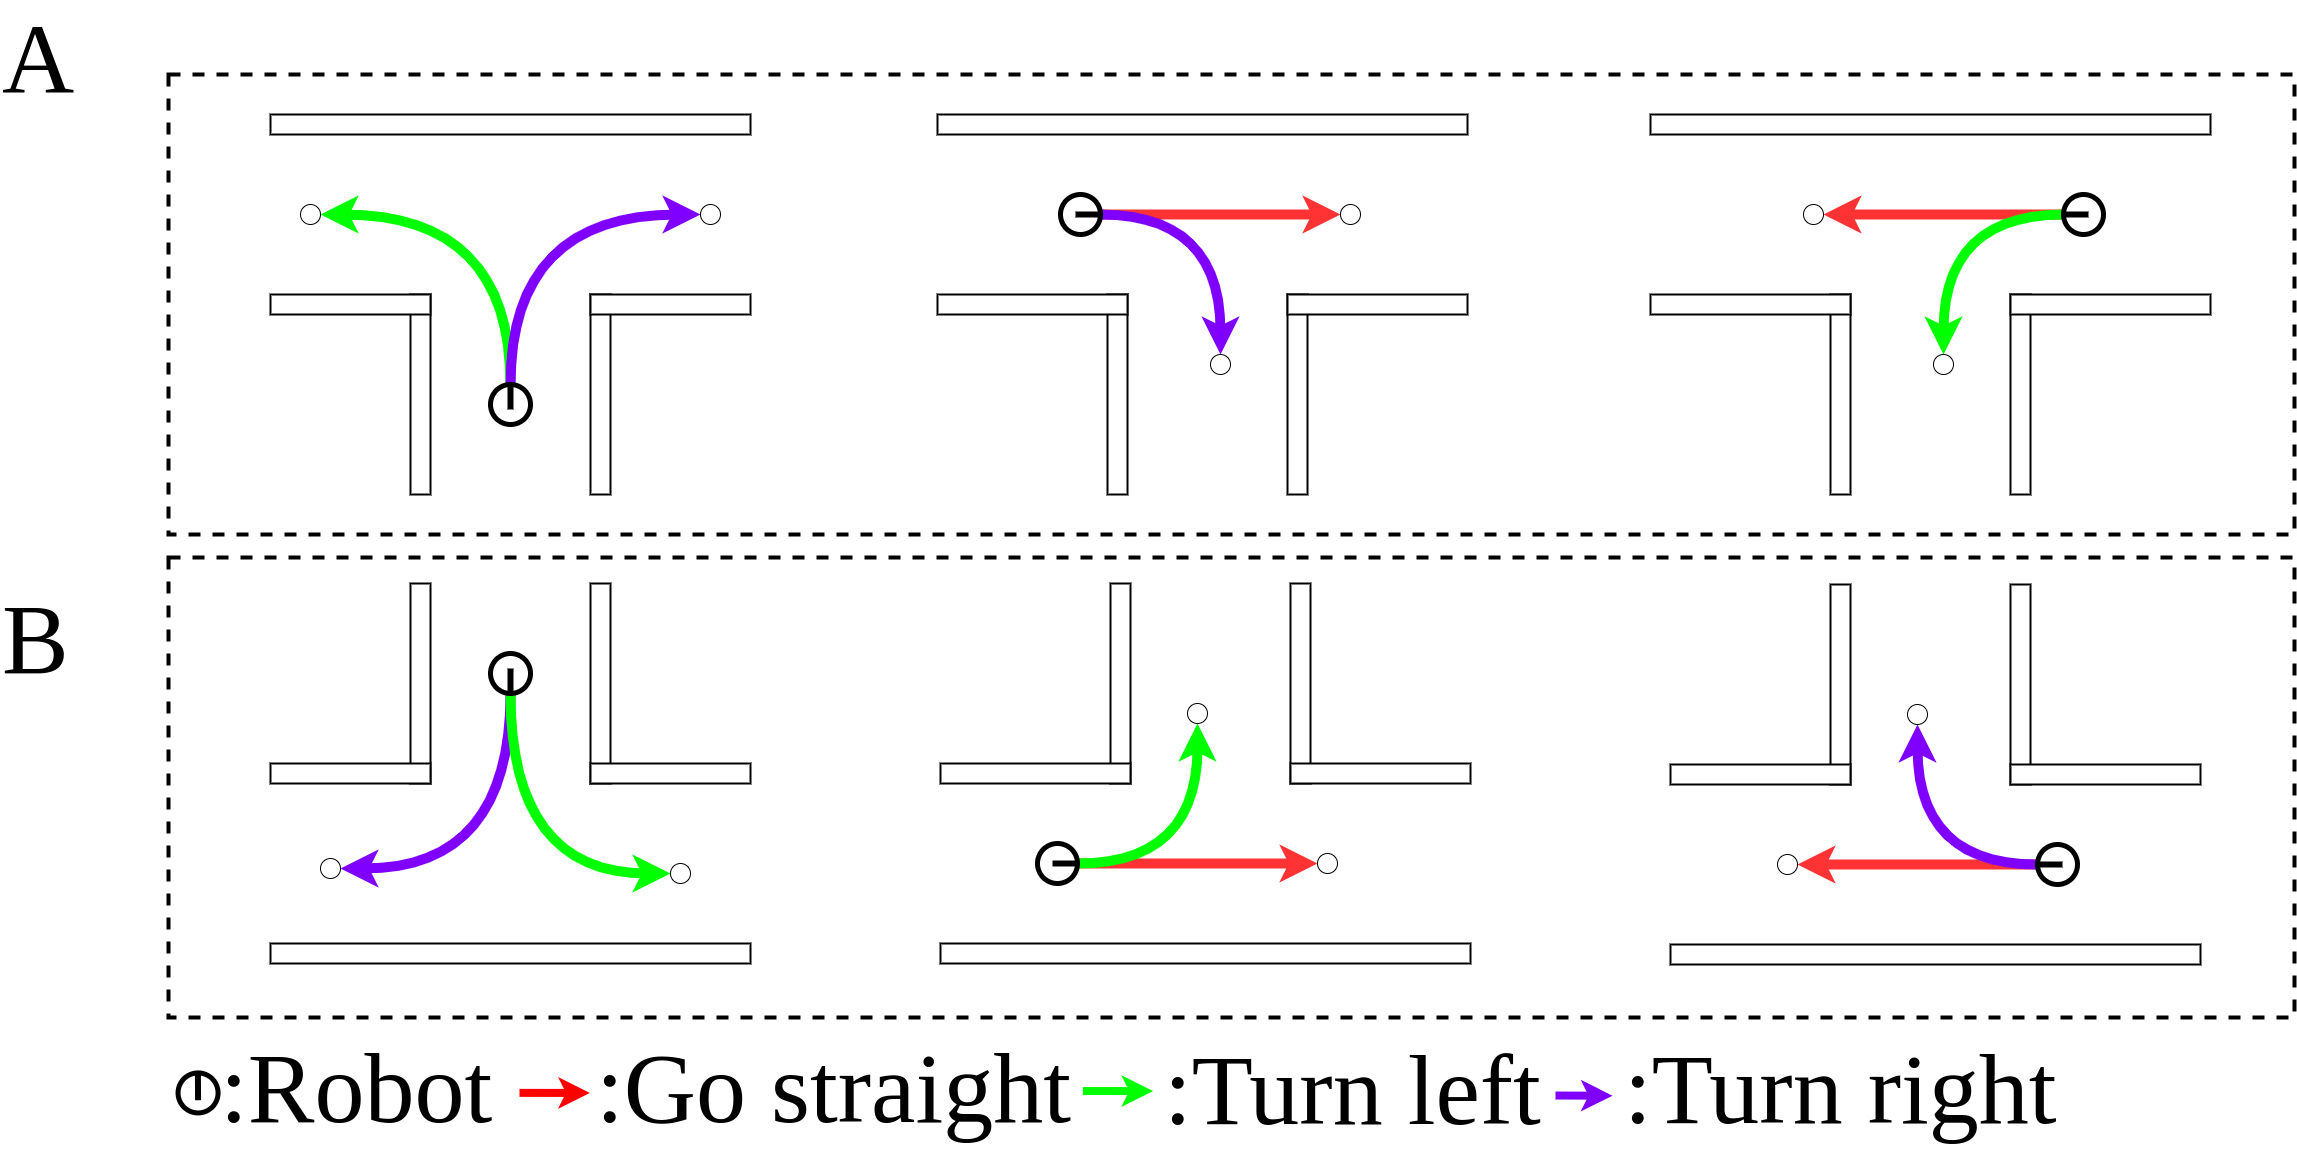
\includegraphics[keepaspectratio, scale=0.15]
      {images/select.png}
 \caption{Moving pattern at points A and B}
 \label{Fig:select}
\end{figure}

全ての走行パターンを網羅するように模倣学習を行うため, \figref{Fig:route}に示すようにaからfまでの経路を繰り返し走行させる. なお, 目標方向はwaypoint\_navから生成され, データセットに加えられる. 学習終了後, テストフェーズに移行するが, 学習時と同様にaからfまでの順番で経路をロボットに走行させる. また, テストフェーズ時にロボットが壁に衝突した場合, 経路の中央にロボットを移動させた後, 走行を再開させる.

\vspace{1cm}

\begin{figure}[hbtp]
  \centering
 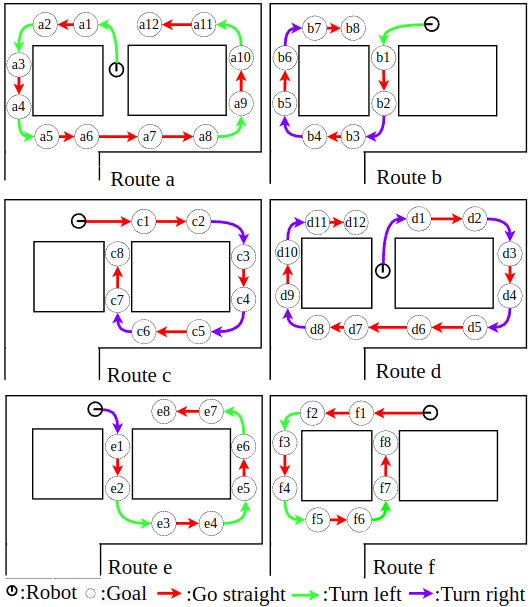
\includegraphics[keepaspectratio, scale=0.6]
      {images/route.png}
 \caption{Moving pattern at points A and B}
 \label{Fig:route}
\end{figure}

\newpage

%!TEX root = ../thesis.tex

\section{課題点と2つのアプローチによる実験}
我々が行ってきた研究では, 簡易的なシミュレータ上で提案手法が有効だと確認されている. そのため, 次の段階として実環境における提案手法の有効性を検証することを試みた. そこで, 新たに顕在化した課題点は以下の2つの点である.

\begin{itemize}
  \item 実験条件(主にカメラ画像に影響を及ぼす光である)を揃える関係上, 実験を行う時間帯を光の変化が少ない夜間に固定する必要があるため, 1日に実験を行える時間が少なく, 1回の学習に何日も費やす必要がある
  \item 長時間の学習に耐えられるだけのバッテリ容量がロボットにない
\end{itemize}

これらの課題点から, 学習時間の短縮が必要であると判断した. そのため, 2つのアプローチを提案し, 学習量を削減する.
\par
この節では, まず, 従来の実験を簡単に紹介する. 次に, 2つのアプローチについての詳細と行った実験を述べる. 最後に, アプローチを試みる前と各アプローチによる実験結果を比較し, 議論を行う.

\subsection{従来の実験}

\begin{itemize}
  \item 実験目的\\
  簡易的なシミュレータ上で, 提案手法の有効性の検証を行う
  \item 実験装置\\
  4.1.1で述べた簡易的なシミュレータ環境とロボットで実験を行った
  \item 実験方法\\
  4.1.2で示した経路を繰り返し走行させる. 学習を60000step実行後, テストフェーズに移行する. テストフェーズで正しい順序で経路を選択し, 走行を行えるか確認する. この一連の流れを10回繰り返し行う.

  \newpage

  \item 実験結果\\
  実験結果を\figref{Fig:60000step}に示す. この図は, それぞれの走行パターンにおいて正しく経路を選択し, 走行できた回数を表している. \tabref{table:result}に全パターンの成功回数を合計した結果を示す. なお, 分母が120であるのはテストフェーズにおいて, 全12パターンからなる経路を走行させ, 評価を行うことを10回繰り返したためである. 
  \par
  \tabref{table:result}に示すように, 目標方向に従って113/120回, 正しい経路を選択する様子が見られた. 

\vspace{1cm}

\begin{figure}[hbtp]
  \centering
 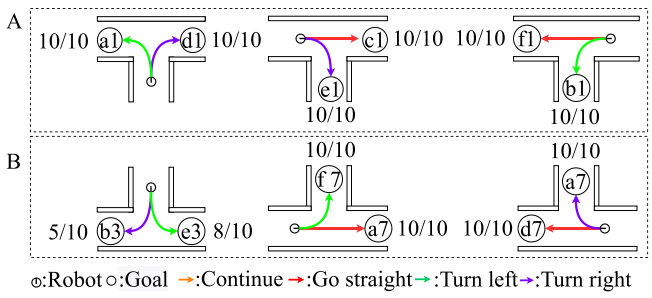
\includegraphics[keepaspectratio, scale=0.5]
      {images/60000step.png}
 \caption{Experimental results for each moving pattern from \cite{mech}}
 \label{Fig:60000step}
\end{figure}

\vspace{1cm}

\begin{table}[hbtp]
  \caption{Experimental results}
  \label{table:result}
  \centering
  \begin{tabular}{|c|c|c|}
    \hline
    Experiments & Step & Total result\\
    \hline
    Conventional & 60000 & 113/120(94.2\%)\\
    \hline
  \end{tabular}
\end{table}

\end{itemize}

\newpage

この従来の実験を基に, 単に60000stepから10000stepに学習量を削減し, 実験した結果を下記に示す.

実験結果を \figref{Fig:10000step} に示す. この図は, それぞれの走行パターンにおいて正しく経路を選択し, 走行できた回数を表している. \tabref{table:result_without} に実験ごとに全パターンの成功回数を合計した結果を示す. \tabref{table:result_without} に示すように, 目標方向に従って 87/120 回, 正しい経路を選択する様子が見られた.

60000stepの実験と成功率を比較すると約22\%ほどの差がある. これでは, 学習量を削減できたとは言い難い. そのため, 後述する2つのアプローチを試みることで成功率の改善を図る.

\vspace{0.5cm}

\begin{figure}[hbtp]
  \centering
 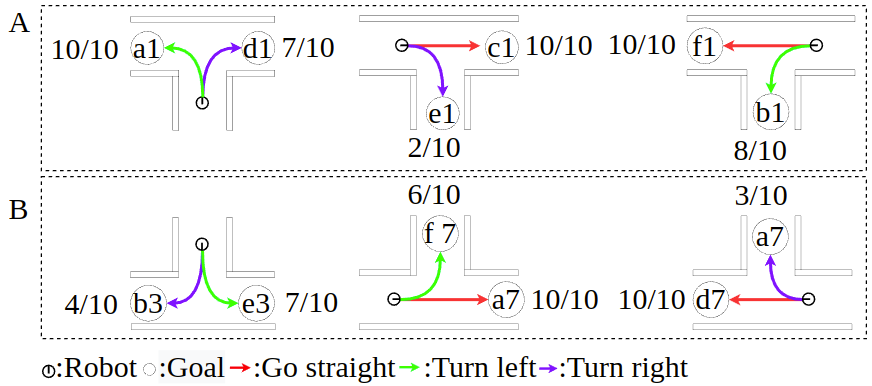
\includegraphics[keepaspectratio, scale=0.43]
      {images/10000step.png}
 \caption{Experimental results for each moving pattern at 10000step by conventional}
 \label{Fig:10000step}
\end{figure}  

\vspace{0.5cm}

\begin{table}[hbtp]
  \caption{Experimental results at 10000step by conventional}
  \label{table:result_without}
  \centering
  \begin{tabular}{|c|c|c|}
    \hline
    Experiments & Step & Total results\\
    \hline
    Conventional & 60000 & 113/120(94.2\%)\\
    \hline
    Conventional & 10000 & 87/120(72.5\%)\\
    \hline
  \end{tabular}
\end{table}

\newpage



\subsection{アプローチ1:データセットに加えるデータの割合変更}
従来の実験における10000stepごとのコマンドに対応するデータ数を\figref{Fig:hist}に示す. \figref{Fig:hist} (a)より, 直進コマンド時のデータ数が圧倒的に多いことがわかる. このデータ数の偏りを解消するため, \figref{Fig:hist} (b)に示すように, 左折と右折コマンドのデータ数を7倍にする. 7倍にするのは, 左折と右折コマンドのデータ数を直進コマンドと同程度にするためである. なお, データ数を何倍にするのが望ましいのか本論文では議論しない. 実験により, データセットに加えるデータ数の割合変更が有効か検証する.

% \begin{figure}[h]
%   \begin{minipage}[b]{0.5\linewidth}
%     \centering
%  \includegraphics[keepaspectratio, scale=0.3]
%       {images/hist_change_org.png}
%  \subcaption{hoge}
%  \label{Fig:hist_org}
% %  \label{Fig:hist_change_org}
% \end{minipage}

%   \begin{minipage}[b]{0.5\linewidth}
%     \centering
%  \includegraphics[keepaspectratio, scale=0.3]
%       {images/hist_change_times7.png}
%  \subcaption{jkofs}
%  \label{Fig:hist_times7}
% %  \label{Fig:hist_change_times7}
%   \end{minipage}
%   \caption{Number of data per command per 10000steps in conventional experiments}
%    \label{Fig:hist}
% \end{figure}

\begin{figure}[h]
  \centering
  \begin{minipage}[b]{67mm}
    \centering
    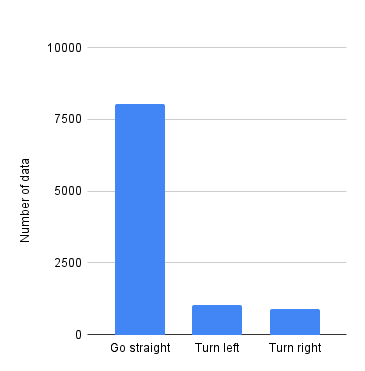
\includegraphics[width=67mm]{images/hist_change_org.png}
    \caption*{(a)}
  \end{minipage} 
  % \newpage
  % \hspace{0.03\columnwidth}
  \begin{minipage}[b]{67mm}
    \centering
    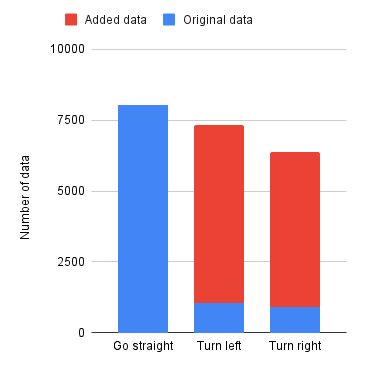
\includegraphics[width=67mm]{images/hist_change_times7.png}
    \caption*{(b)}
  \end{minipage}
  \caption{Number of data per command per 10000steps in conventional experiments}
  \label{Fig:hist}
\end{figure}

\begin{itemize}
  % \item 実験目的\\
  % データセットに加えるデータの割合変更が有効か検証を行う
  \item 実験装置\\
  4.1.1で述べた簡易的なシミュレータ環境とロボットで実験を行った
  \item 実験方法\\
  4.1.2で示した経路を繰り返し走行させる. 学習を10000step実行後, テストフェーズに
  移行する. テストフェーズで正しい順序で経路を選択し, 走行を行えるか確認する. こ
  の一連の流れを10回繰り返し行う.
  \newpage
  \item 実験結果\\
  実験結果を\figref{Fig:10000step_act1.0}に示す. この図は, それぞれの走行パターンにおいて正しく経路を選択し, 走行できた回数を表している. \tabref{table:result3}に実験ごとに全パターンの成功回数を合計した結果を示す. 
  \tabref{table:result3}に示すように, 目標方向に従って99/120回, 正しい経路を選択する様子が見られた. 
  \par
  60000stepの実験と成功率を比較すると約12\%ほど差があり, アプローチ1を試みた結果では成功率が十分だとは言い難い. 次に成功率を改善するため, 後述するアプローチ2を試みた.

  \vspace{0.5cm}

  \begin{figure}[hbtp]
    \centering
   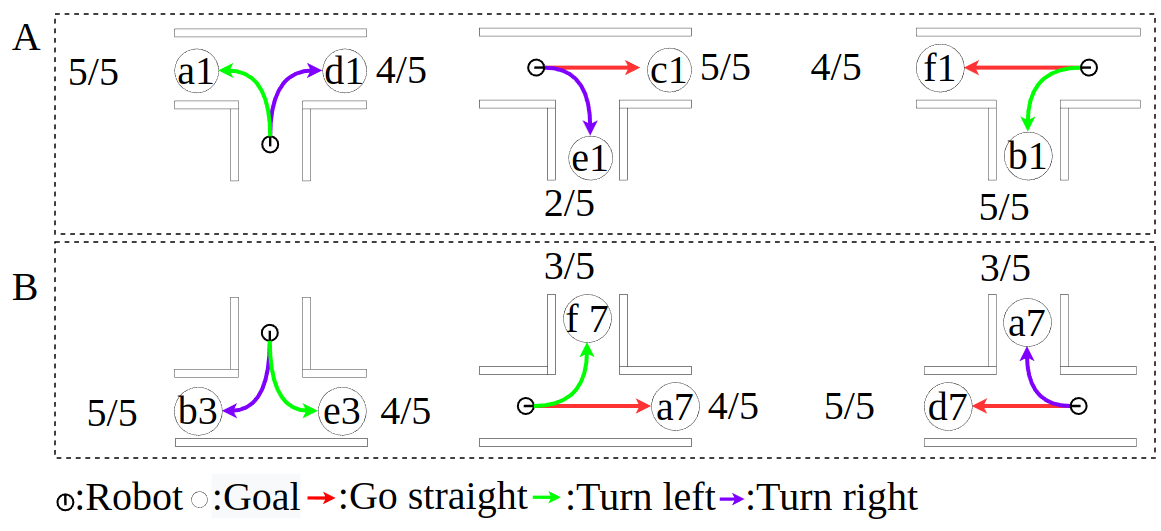
\includegraphics[keepaspectratio, scale=0.5]
        {images/10000step_act1.0.png}
   \caption{Experimental results for each moving pattern by Approach1}
   \label{Fig:10000step_act1.0}
  \end{figure}  
  
  \vspace{0.5cm}

  \begin{table}[hbtp]
    \caption{Experimental results by Approach 1}
    \label{table:result3}
    \centering
    \begin{tabular}{|c|c|c|}
      \hline
      Experiments & Step & Total results\\
      \hline
      Conventional & 60000 & 113/120(94.2\%)\\
      \hline
      Conventional & 10000 & 87/120(72.5\%)\\
      \hline
      Approach1 & 10000 & 99/120(82.5\%)\\
      \hline
    \end{tabular}
  \end{table}

\end{itemize}

\newpage

\subsection{アプローチ2:学習フェーズにおける積極的な蛇行}
清岡ら\cite{kiyooka}により, 目標経路上に加えて離れた状態を学習することが, テストフェーズでの走行に大きな影響を与えるため, 重要だとされている. そのため, より積極的に蛇行を行い, 目標経路から離れた状態を増加させることを検討する. \par
実験で用いているシステムの学習フェーズでは,  \figref{Fig:act1.0}に示すようにロボットが目標経路上付近を走行している場合, 訓練中の学習器へ画像を入力し, 出力される角速度を用いて走行している. この場合に, 目標経路から一定の距離離れると地図を用いたルールベース制御器の走行に切り替わり, 強制的にロボットを目標経路上に戻すように制御を行う. 

\begin{figure}[hbtp]
  \centering
 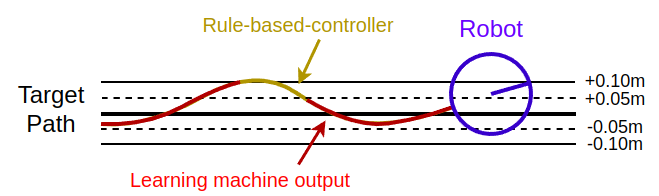
\includegraphics[keepaspectratio, scale=0.58]
      {images/act1.0.png}
 \caption{Moving on the target path}
 \label{Fig:act1.0}
\end{figure}

訓練中の学習器へ画像を入力し, \figref{Fig:3action}のように出力される角速度を1.5倍にする. その結果, \figref{Fig:act1.5}に示すように蛇行する頻度が高くなり, 目標経路から離れた状態をより多く学習できる可能性がある. なお, 得られた角速度を何倍にするのが望ましいのか本論文では議論しない. 実験により, 学習フェーズにおける積極的な蛇行が有効か検証する.

\begin{figure}[hbtp]
  \centering
 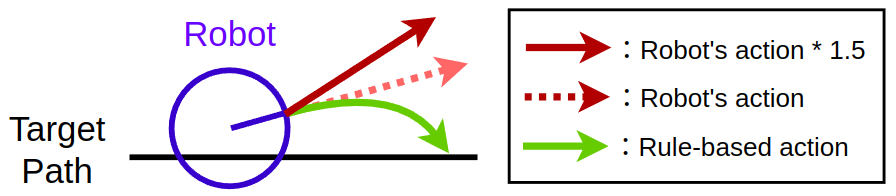
\includegraphics[keepaspectratio, scale=0.43]
      {images/3action.png}
 \caption{Robot behavior}
 \label{Fig:3action}
\end{figure}

\begin{figure}[hbtp]
  \centering
 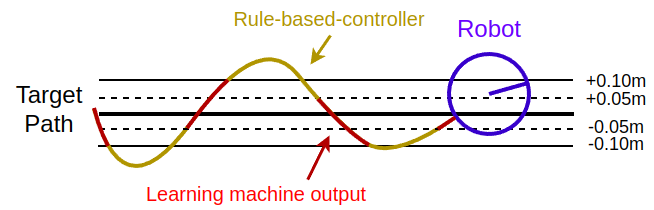
\includegraphics[keepaspectratio, scale=0.58]
      {images/act1.5.png}
 \caption{Moving on the target path attempting approach 2}
 \label{Fig:act1.5}
\end{figure}

\begin{itemize}
  % \item 実験目的\\
  % データセットに加えるデータの割合変更が有効か検証を行う
  \item 実験装置\\
  4.1.1で述べた簡易的なシミュレータ環境とロボットで実験を行った
  \item 実験方法\\
  4.1.2で示した経路を繰り返し走行させる. 学習を10000step実行後, テストフェーズに
  移行する. テストフェーズで正しい順序で経路を選択し, 走行を行えるか確認する. こ
  の一連の流れを10回繰り返し行う.
  \item 実験結果\\
  実験結果を\figref{Fig:10000step_act1.5}に示す. この図は, それぞれの走行パターンにおいて正しく経路を選択し, 走行できた回数を表している. \tabref{table:result4}に実験ごとに全パターンの成功回数を合計した結果を示す. 
  \tabref{table:result4}に示すように, 目標方向に従って109/120回, 正しい経路を選択する様子が見られた. 
  % また, 
  % \par
  % \tabref{table:result4}からアプローチ1の実験より, 成功率が改善していることがわかる. また, 60000stepの実験と成功率を比較した場合, 約4\%ほどの差がある. これには, 以下2つの要因が挙げられる.
  % \begin{itemize}
  %   \item 
  % \end{itemize}
  % そのため, 10000stepから20000stepに学習量を増加し, 実験した結果を下記に示す.

  
  \begin{figure}[hbtp]
    \centering
   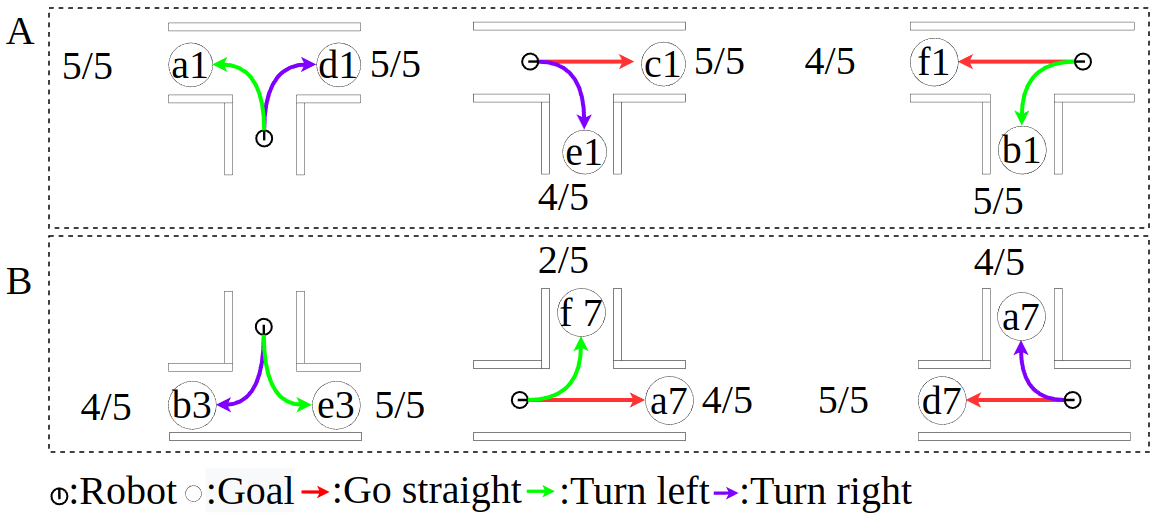
\includegraphics[keepaspectratio, scale=0.55]
        {images/10000step_act1.5.png}
   \caption{Experimental results for each moving pattern at 10000step by Approach 1+2}
   \label{Fig:10000step_act1.5}
  \end{figure}  
  
  % \vspace{0.5cm}

  \begin{table}[hbtp]
    \caption{Experimental results at 10000step by Approach 1+2}
    \label{table:result4}
    \centering
    \begin{tabular}{|c|c|c|}
      \hline
      Experiments & Step & Total results\\
      \hline
      Conventional & 60000 & 113/120(94.2\%)\\
      \hline
      Conventional & 10000 & 87/120(72.5\%)\\
      \hline
      Approach1 & 10000 & 99/120(82.5\%)\\
      \hline
      \textbf{Approach1+2} & \textbf{10000} & \textbf{109/120(90.8\%)}\\
      \hline
    \end{tabular}
  \end{table}

  % \vspace{1cm}

  \tabref{table:result4}からアプローチ1の実験より, 成功率が改善していることがわかる. また, 60000stepの実験と成功率を比較した場合, 約3\%ほどの差がある. 
  % \tabref{table:factor}
  以下に\figref{Fig:10000step_act1.5}における成功率が低い場所と要因を示す.
  \begin{itemize}
    \item f7\\
    4.1.2で示した経路の最後であり, 学習フェーズが終了する直前の三叉路である. そのため, データセットにf7のデータが加えられてから十分な学習ができていない
    \item a7, b3, e1\\
    これらは, 全て右折する場所である. \figref{Fig:hist}より, 他のコマンドのデータと比較して右折コマンドのデータが少ないことがわかる. このことから, 右折コマンドのデータを十分に学習できていない
  \end{itemize} 

  この2つの点から, 学習量を増加すると成功率が改善する可能性がある. そのため, 10000stepから20000stepに学習量を増加した実験結果を後述する.

  \newpage

  % \begin{table}[hbtp]
  %   \caption{Experimental results}
  %   \label{table:factor}
  %   \centering
  %   \begin{tabular}{|c|c|}
  %     \hline
  %     Points with low success rates & Primary factor\\
  %     \hline
  %     f7 & It is the last of the paths shown in 4.1.2, and the learning phase is terminated after passing through f7. Therefore, the data set has not been fully trained since the data of f7 was added to the dataset\\
  %     \hline
  %     a7, b3, e1 & 10000\\
  %     \hline
  %   \end{tabular}
  % \end{table}

  学習フェーズにおける目標経路からの距離によるデータの割合を\figref{Fig:hist_act_training}に示す. \par
  この図から, 学習器から得られた角速度を1.5倍にした場合, データの割合が目標経路付近では減少し, 目標経路から離れた場所では増加している. よって, アプローチ2を試みた結果, 学習フェーズでは目標経路から離れる行動が増えた. すなわち, 積極的に蛇行している可能性が高い.

  % \vspace{1cm}

  \begin{figure}[hbtp]
    \centering
   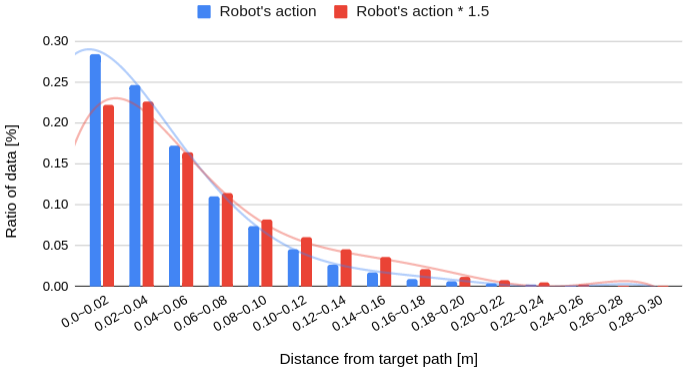
\includegraphics[keepaspectratio, scale=0.37]
        {images/hist_act_training.png}
   \caption{Ratio of data by distance from target path in learning phase}
   \label{Fig:hist_act_training}
  \end{figure}  

  % \newpage

  テストフェーズにおける目標経路からの距離によるデータの割合を\figref{Fig:hist_act_test}に示す. この図から, 学習器から得られた角速度を1.5倍にした場合, データの割合が目標経路付近では増加し, 目標経路から離れた場所では減少している. よって, アプローチ2を試みた結果, テストフェーズでは目標経路付近の行動が増えた. すなわち, アプローチ2を試みる前に比べ, より正確に経路追従行動を模倣している可能性が高い.

  \begin{figure}[hbtp]
    \centering
   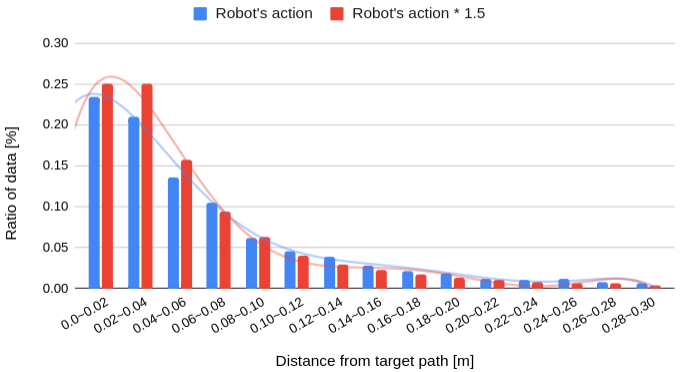
\includegraphics[keepaspectratio, scale=0.37]
        {images/hist_act_test.png}
   \caption{Ratio of data by distance from target path in test phase}
   \label{Fig:hist_act_test}
  \end{figure}  

  % \newpage

\end{itemize}

アプローチ1,2の実験を基に, 単に10000stepから20000stepに学習量を増やし, 実験した結果を下記に示す.

\figref{Fig:20000step_act1.5}は, それぞれの走行パターンにおいて正しく経路を選択し, 走行できた回数を表している. \tabref{table:result5} に実験ごとに全パターンの成功回数を合計した結果を示す. \tabref{table:result5} に示すように, 目標方向に従って 114/120 回, 正しい経路を選択する様子が見られた. また, 成功率が60000stepの実験と同程度になった. このことから, アプローチ1+2によって学習量が約67\%削減でき, 実験を実環境に移す際の問題が解決できたといえる. 

\begin{figure}[hbtp]
  \centering
 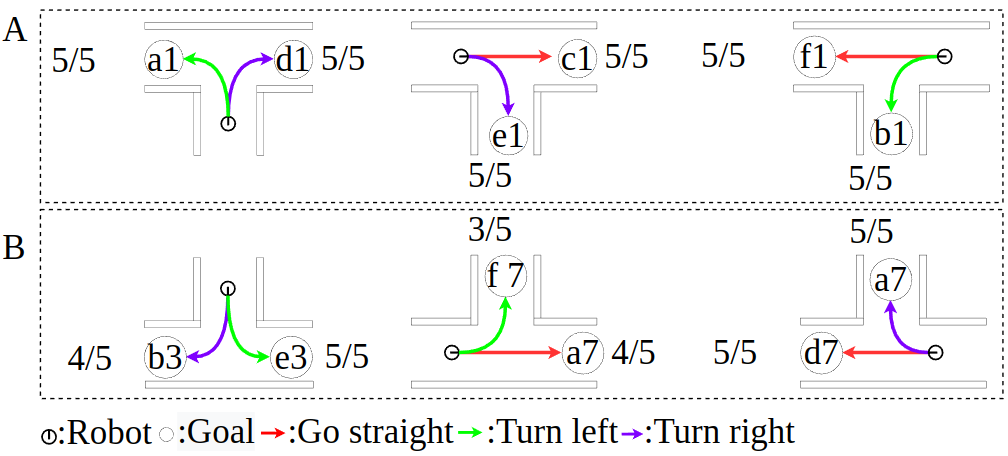
\includegraphics[keepaspectratio, scale=0.42]
      {images/20000step_act1.5.png}
 \caption{Experimental results for each moving pattern at 20000step by Approach 1+2}
 \label{Fig:20000step_act1.5}
\end{figure} 

\begin{table}[hbtp]
  \caption{Experimental results at 20000step by Approach 1+2}
  \label{table:result5}
  \centering
  \begin{tabular}{|c|c|c|}
    \hline
    Experiments & Step & Total results\\
    \hline
    Conventional & 60000 & 113/120(94.2\%)\\
    \hline
    Conventional & 10000 & 87/120(72.5\%)\\
    \hline
    Approach1 & 10000 & 99/120(82.5\%)\\
    \hline
    Approach1+2 & 10000 & 109/120(90.8\%)\\
    \hline
    \textbf{Approach1+2} & \textbf{20000} & \textbf{114/120(95\%)}\\
    \hline
  \end{tabular}
\end{table}

\newpage

%

%
%% Main Matter
\mainmatter{}
%
\chapter{序論}
\label{chap:introduction}
%
%\input{introduction/preface}
%
%!TEX root = ../thesis.tex

\section{背景}
近年, 機械学習を用いた自律走行に関する研究が盛んにされており, その中でカメラ画像を用いてロボットへ自律走行を行わせる研究もされている. Bojarskiら\cite{bojarski}は\figref{Fig:bojarski_train}に示すシステムで, 人間のドライバーが操作するステアリング角度と前方カメラ画像を用いて模倣学習を行った. また, \figref{Fig:bojarski_test}に示すように, 訓練したネットワークに画像を入力し, 生成される操舵指令を用いて走行を行う手法を提案した.

\vspace{0.5cm}

\begin{figure}[hbtp]
  \centering
 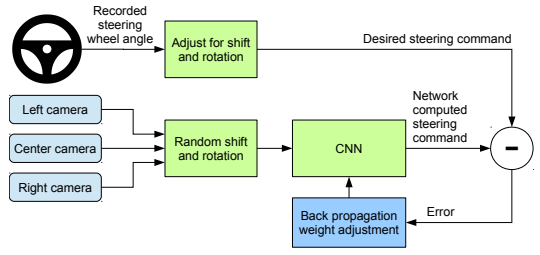
\includegraphics[keepaspectratio, scale=0.9]
      {images/bojarski_train.png}
 \caption{Training the neural network from \cite{bojarski}}
 \label{Fig:bojarski_train}
\end{figure}

\begin{figure}[hbtp]
     \centering
    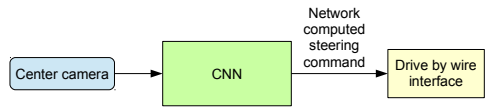
\includegraphics[keepaspectratio, scale=0.7]
         {images/bojarski_test.png}
    \caption{The trained network is used generate steering commands from a single front-facing center camera from \cite{bojarski}}
    \label{Fig:bojarski_test}
\end{figure}

\newpage

本研究室においても, 岡田ら\cite{okada1}\cite{okada2}は\figref{Fig:okada_structure}に示すようなシステムを用いて\figref{Fig:okada_nav}のように経路追従行動を模倣学習し, カメラ画像に基づいた経路追従行動を獲得した. このシステムでは, LiDAR, オドメトリを入力としたルールベース制御器(後述する”地図を用いたルールベース制御器”)による経路追従行動を前方カメラ画像を用いてend-to-endで模倣学習した. 

\vspace{2.5cm}

\begin{figure}[hbtp]
     \centering
     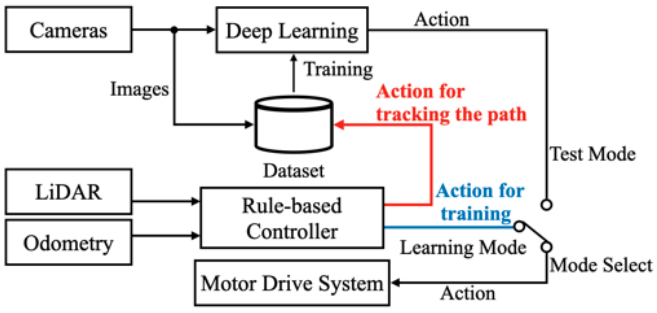
\includegraphics[keepaspectratio, scale=0.55]
          {images/okada_structure.png}
     \caption{Structure of the proposed system from \cite{okada1}}
     \label{Fig:okada_structure}
\end{figure}

\begin{figure}[hbtp]
     \centering
    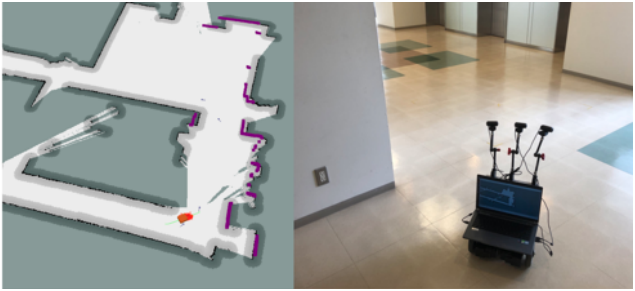
\includegraphics[keepaspectratio, scale=0.5]
         {images/okada_nav.png}
    \caption{A robot that follows a path using vision based on the proposed method from \cite{okada1}}
    \label{Fig:okada_nav}
\end{figure}

\newpage

上記の研究により, カメラ画像に基づいてロボットが学習した経路を周回可能であることが確認されている. 次に岡田らの研究(以下, 「従来手法」と称する)をベースに, \figref{Fig:road}のような分岐路において, 任意の経路を選択する機能の追加を検討する.

\vspace{1cm}

\begin{figure}[hbtp]
     \centering
    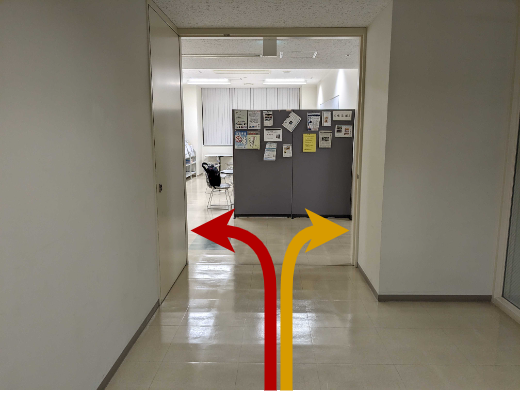
\includegraphics[keepaspectratio, scale=0.5]
         {images/road.png}
    \caption{A fork in the road where the direction of travel is not unique}
    \label{Fig:road}
\end{figure}

\newpage

本研究では, 従来手法をベースに「直進」, 「左折」, 「右折」の目標とする進行方向の情報(以下, 「目標方向」と称する)をデータセットと学習器へ与える. これにより, 訓練済みの学習器の出力を用いた走行において, 目標方向により任意の経路を選択可能とする機能の追加を提案する. 提案手法全体の流れを\figref{Fig:suggest_work}に示す. 

\begin{figure}[hbtp]
     \centering
    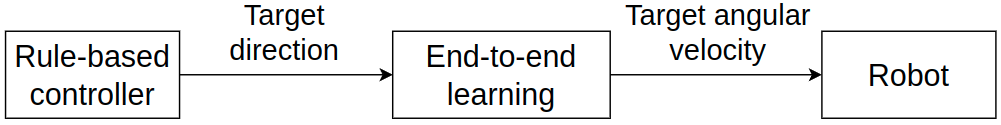
\includegraphics[keepaspectratio, scale=0.38]
         {images/suggest_work.png}
    \caption{Overall flow of the proposed method}
    \label{Fig:suggest_work}
\end{figure}

最終的にはカメラ画像を入力として, トポロジカルマップによって生成される目標方向に従って, 目的地まで移動する自律走行の手法を提案することを検討する. トポロジカルマップとは\figref{Fig:tsudanuma}に示すように, 重要な情報のみを残し, 分岐路などの目印(ノード)とつながり(エッジ)を持つ簡略化された地図である.

\vspace{0.5cm}

\begin{figure}[hbtp]
     \centering
    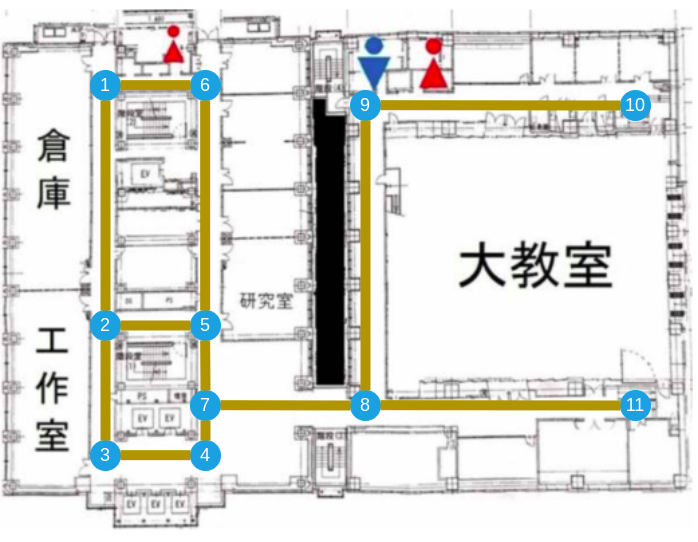
\includegraphics[keepaspectratio, scale=0.45]
         {images/tsudanuma.png}
    \caption{Topological map}
    \label{Fig:tsudanuma}
\end{figure}

カメラ画像とステアリング角度に, 条件を加えて学習を行う条件付き模倣学習によって, 自律移動を行う研究を述べる. Felipeら\cite{felipe}は前方カメラ画像, ステアリング角度, 加速度と「continue」, 「left」, 「straight」, 「right」からなるコマンドを入力とした\figref{Fig:felipe_network}のようなネットワークを用いて, \figref{Fig:felipe}に示すような実環境と都市環境のシミュレータ上で, 模倣学習のテスト時においてもコマンドによって制御可能であることを確認している.

\vspace{0.5cm}

\begin{figure}[hbtp]
     \centering
    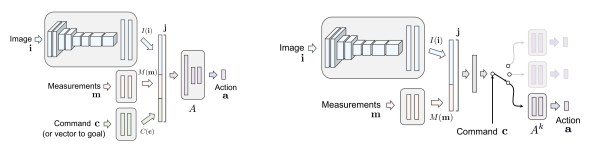
\includegraphics[keepaspectratio, scale=0.65]
         {images/felipe_network.png}
    \caption{Two network architectures for command-conditional imitation learning from \cite{felipe}}
    \label{Fig:felipe_network}
\end{figure}

\vspace{0.5cm}

\begin{figure}[hbtp]
     \centering
    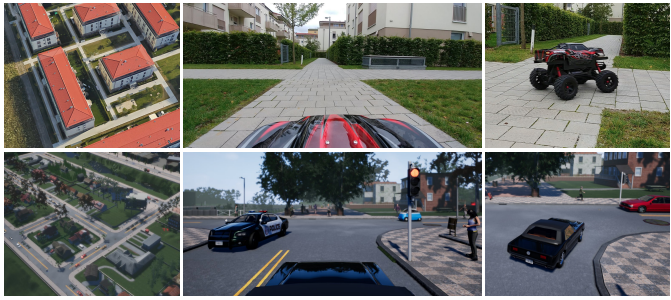
\includegraphics[keepaspectratio, scale=0.57]
         {images/felipe.png}
    \caption{End-to-end driving via conditional imitation learning from \cite{felipe}}
    \label{Fig:felipe}
\end{figure}

\newpage

また, Hawkeら\cite{hawke}は\figref{Fig:hawke}のような, 3つの前方カメラ画像と「go-straight」, 「turn-left」, 「turn-right」からなるコマンドを入力とする構造のモデルを用いて, 実環境での複雑な都市環境というシナリオで, 意思決定が可能なモデルをわずか30時間の学習データで学習可能であることを示している.

\vspace{3cm}

\begin{figure}[hbtp]
     \centering
    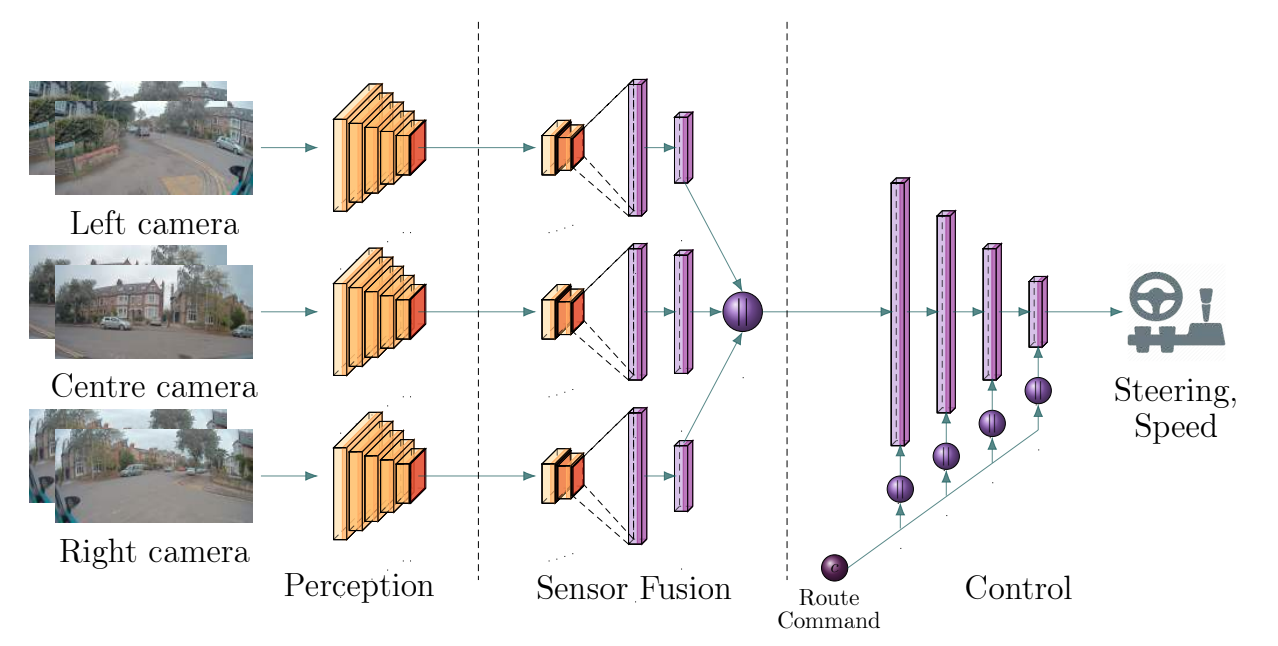
\includegraphics[keepaspectratio, scale=0.3]
         {images/hawke.png}
    \caption{Model structure from \cite{hawke}}
    \label{Fig:hawke}
\end{figure}

\newpage
%!TEX root = ../thesis.tex

\section{目的}
本研究では, 経路追従行動を模倣学習し, カメラ画像に基づいた経路追従行動を獲得する手法である岡田らの従来手法をベースとして, 分岐路において「直進」, 「左折」などのコマンドによる制御で任意の経路を選択可能にする機能の追加を提案する. また, シミュレータ上での実験を実環境に移す際に, 問題となった学習時間の長さについて, 2 つのアプローチの提案と検証を行った. さらに, 実環境における提案手法の有効性を検証することを目的とする.

% \begin{figure}[hbtp]
%   \centering
%  \includegraphics[keepaspectratio, scale=0.8]
%       {images/RaspberryPiMouse.png}
%  \caption{Example}
%  \label{Fig:Example}
% \end{figure}

% \newpage

%!TEX root = ../thesis.tex

\section{論文構成}
1章では, 本研究における背景,  及び目的を述べた. 2章では, 本研究で用いた深層学習の他所技術とベースとする従来手法について述べる. 3章では, 従来手法をベースにした, 提案手法を述べる. 4章では, シミュレータと実環境での実験を行う. 5章では, 本研究の結論を述べる.

% \begin{figure}[hbtp]
%   \centering
%  \includegraphics[keepaspectratio, scale=0.8]
%       {images/RaspberryPiMouse.png}
%  \caption{Example}
%  \label{Fig:Example}
% \end{figure}

\newpage

%

\chapter{要素技術}
\label{chap:element_technology}
%
%\input{introduction/preface}
%
%!TEX root = ../thesis.tex

\section{ナビゲーション}\label{sec:navigation-stack}
LiDARやオドメトリなどのセンサ情報を利用して自律走行する移動ロボットの多くは,ROS Navigation stack\cite{nav1,nav2}を採用している.例えば,つくば市内の遊歩道を移動ロボットが自律走行する技術チャレンジ「つくばチャレンジ」において,原らの技術調査\cite{robomech2024-hara}によると,少なくとも参加76チーム中22チームが自律走行でROS Navigation stack使用していたと報告されている.これは,オープンソースのソフトウェアにとしては最多の利用数であった.ROS Navigation stackには,以下の主要な機能が含まれている.

\begin{itemize}
     \item \textbf{自己位置推定(Localization)}\\
     AMCL(Adaptive Monte Carlo Localization)アルゴリズムを用いて,ロボットの現在位置を推定する.
     \item \textbf{地図生成(Mapping)}\\
     SLAM(Simultaneous Localization and Mapping)技術を活用し,環境のマッピングを行う.
     \item \textbf{経路計画(Path Planning)}\\
     Dijkstra法\cite{dijkstra2022note}やA*アルゴリズム\cite{hart1968formal-astar}を用いて,最適経路を計画する.
     \item \textbf{障害物回避(Obstacle Avoidance)}\\
     センサデータに基づいて障害物を検知し,動的に回避しながら移動する.
\end{itemize}

\newpage

%!TEX root = ../thesis.tex

\section{ニューラルネットワーク}
ニューラルネットワーク(Neural Network)は,人間の脳の神経回路に着想を得た計算モデルであり,機械学習や人工知能の分野で重要な役割を果たしている.大量のデータから学習し,パターン認識や予測などの複雑なタスクを遂行する能力を持つ.パーセプトロンを入れる

ニューラルネットワークは,多数のノード(ニューロン)が層状に接続された構造を持つ.各ノードは,入力信号を受け取り,重み付けを行い,活性化関数を適用することで出力信号を生成する.これらのノードは,入力層,隠れ層,出力層の3つの層に分けられる.

\begin{itemize}
     \item 入力層\\
     入力データを受け取る層であり,各ノードは入力データの各特徴に対応する.
     \item 隠れ層\\
     入力層と出力層の間にある層であり,複数の隠れ層を持つことができ,複雑な非線形関係を学習することが可能になる.
     \item 出力層\\
     ネットワークの最終的な出力を生成する層である.
\end{itemize}

各層のノードは,次の層のノードと接続されており,接続には重みが割り当てられている.学習プロセスでは,これらの重みを調整することで,ネットワークが目的のタスクを実行できるように最適化される.
% この最適化は,一般的に損失関数を最小化するように,勾配降下法などの最適化アルゴリズムを用いて行われる.
多層構造を持つことで,複雑なパターンや特徴を学習し,従来では困難であった高精度な予測を実現した学習手法を深層学習と呼ぶ.深層学習は,画像認識,自然言語処理,音声認識といった多岐にわたる分野で活用されており,YOLO\cite{redmon2016you-yolo}やChatGPT\cite{radford2018improving-gpt, radford2019language-gpt,brown2020language-gpt}などの成功例が多数存在し,高い性能が評価されている.

\begin{figure}[hbtp]
     \centering
    \includegraphics[keepaspectratio, scale=0.5]
         {images/RaspberryPiMouse.png}
    \caption{Neural Network}
    \label{Fig:MLP}
\end{figure}   

\newpage

%

\chapter{提案手法}
\label{chap:proposed_method}
%
%\input{introduction/preface}
%
%!TEX root = ../thesis.tex

\section{本章の概要}

本章では,2章で述べたようにロボットの行動を考慮した歩行者の軌道予測を行う手法を提案する.学習に用いたアルゴリズムに関する内容を3.2章,

% 以下では,予測を行うネットワーク構造とその学習方法に関して説明する.

% 〜について目指す.〜について提案する.

\section{問題設定}
本論文における歩行者のグラフ表現を説明する.時刻$t$におけるシーン内の歩行者の位置を表す空間グラフを$G_t = (V_t, E_t)$と定義する.ここで,$V_t = \{ v^i_t \mid i = 1, \dots N \}$はグラフ$G_t$のノードの集合であり,各ノード$v^i_t$は$i$番目の歩行者の位置$(x^i_t, y^i_t)$を属性として持つ.$E_t = \{ e^{ij}_t \mid i, j = 1, \dots N \}$はグラフ$G_t$のエッジの集合であり,$e^{ij}_t$はノード$v^i_t$と$v^j_t$が接続されている場合1,そうでない場合0の値をとる.

人間の軌道予測は,歩行者の将来の2次元空間の$x,y$座標を,事前観測の情報を与えて予測ステップ分出力することである.
ここで,歩行者$i$の各時刻の位置を
\begin{equation}
  V_t = \{ v^i_t = (x^i_t, y^i_t) \in \mathbb{R}^2 \mid i = 1, \dots N \}
\end{equation}
と表す.また,$t_{obs}$を観測時間としたとき,観測された全歩行者の位置データを
\begin{equation}
  V_{obs} = \{ V_t \mid t = 1, \dots t_{obs} \}  
\end{equation}
と表す.ここで,時刻$t$の2次元空間における歩行者$i$の位置の確率分布を
\begin{equation}
  \hat{V}_t = \{ \hat{p}^i_t = (\hat{x}^i_t, \hat{y}^i_t) \mid i = 1, \dots N \} \label{hat-pos}
\end{equation}
と表す.$t_{pred}$を予測時間としたとき,予測する全歩行者の位置データを
\begin{equation}
  V_{pred} = \{ \hat{V}_t \mid t = t_{obs + 1}, \dots t_{pred} \}
\end{equation}
と表すことができる.$p^i_t$が$\mathcal{N}(\mu^i_t, \sigma^i_t, \rho^i_t)$となる2変量ガウス分布に従うと仮定する.すなわち,$\hat{p}^i_t$は平均$\hat{\mu}^i_t$,分散$\hat{\sigma}^i_t$,相関係数$\hat{\rho}^i_t$を持つガウス分布
\begin{equation}
  \hat{p}^i_t \sim \mathcal{N}(\hat{\mu}^i_t, \hat{\sigma}^i_t, \hat{\rho}^i_t)
\end{equation}
に従う.ここで,平均を$\hat{\mu}^i_t = (\hat{\mu}^i_{x, t}, \hat{\mu}^i_{y, t})$,分散を$\hat{\sigma}^i_t = (\hat{\sigma}^i_{x, t}, \hat{\sigma}^i_{y, t})$とする.

\section{ネットワーク構造}
本手法で用いられるネットワークは,エンコーダ・デコーダ構造で構成されている.ネットワークは,主にエンコーダモジュール,グラフアテンションネットワークモジュール,デコーダモジュールから構成される.エンコーダモジュールでは,入力データから特徴量を抽出し,グラフアテンションネットワークを用いて,ノード間の関係性を学習する.これらの潜在表現を基に,デコーダモジュールで目的のシーケンス長の予測を行う.
\figref{Fig:network}は,このネットワークの概要を表している.

\begin{figure}[hbtp]
  \centering
 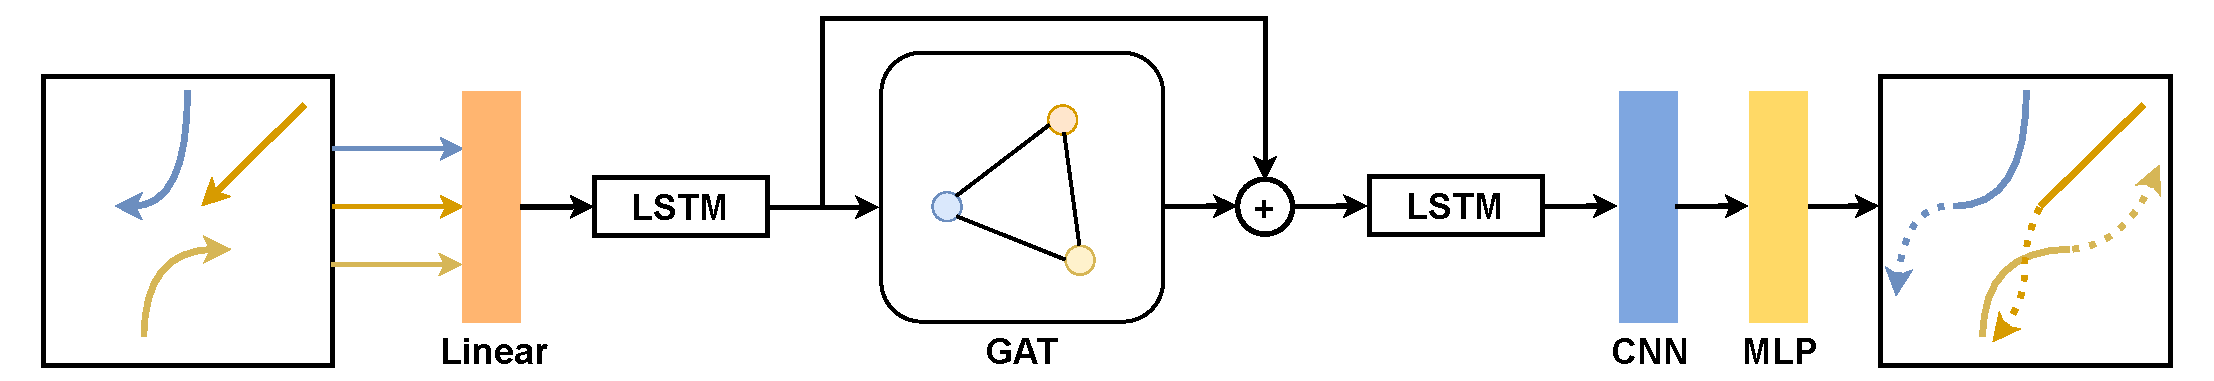
\includegraphics[keepaspectratio, scale=0.36]
      {images/network-comp.pdf}
 \caption{Network Structure}
 \label{Fig:network}
\end{figure}   

\subsection{エンコーダモジュール}
エンコーダでは,まず,入力の各時刻における歩行者の過去の位置は,線形変換層$\phi_{emb}$を用いて高次元空間に埋め込まれる.この埋め込み表現は,LSTM層に入力され,歩行者の過去の位置情報を時間的に処理し,隠れ状態を出力する.隠れ状態は,歩行者の過去の動きを要約したものであり,次のグラフアテンションネットワークに渡される.エンコーダでの処理を式\eqref{emb},\eqref{lstm-en}に示す.なお,$v^i_t \text{と} v^t_i$は等価である.
\begin{align}
  e^t_i &= \phi_{emb}(v^t_i ; W_{emb}) \label{emb} \\
  h_i &= \text{LSTM}_{en}(e^t_i, h^{t-1}_i ; W_{en}) \label{lstm-en}
\end{align}

\subsection{グラフアテンションネットワーク}
ネットワークの中核を担うグラフアテンションネットワーク(GAT)\cite{velickovic2017graph-gat}は,複数層で構成される.各GAT層は,マルチヘッドアテンション機構を用いて,各ノードの特徴をその近傍ノードの特徴と集約する.アテンション機構は,ノード間の関係の強さに基づいて重み付けを行うため,より関連性の高いノードからの情報が強調される.本ネットワークでは,複数のGAT層を積み重ねることで,グラフ構造における高次の依存関係を捉えることができる.各タイムステップにおいて,対応する隣接行列を用いてグラフ畳み込みが実行され,動的なグラフ構造の変化にも対応できる.

歩行者$i$の隠れ状態$h_i$が与えられたとき,全ての歩行者に対して,複数のGAT層を適用する.各層は以下のように適用される.式\eqref{gat-eij}は,ノード$i$に対するノード$j$の特徴の重要度を表している.$W$は重み行列であり,$a$は共有アテンション機構である.また,$\sigma$は活性化関数であり,本手法ではネットワーク全体でPReLU\cite{he2015delving-prelu}を用いた.
\begin{align}
  e_{ij} = a(Wh_i, Wh_j) \label{gat-eij} \\
  \alpha_{ij} = \text{softmax}_{j}(e_{ij}) \\
  h'_i = \sigma\Bigg(\sum_{j \in \mathcal{N}_i} \alpha_{ij}Wh_j \Bigg)
\end{align}

\subsection{デコーダモジュール}
GAT層からの出力は,デコーダモジュールによって将来の歩行者の予測位置に変換される.まず,2つ目のLSTM層がGATによって生成された時空間特徴表現をさらに時間的に処理する.次に,1次元畳み込み層を用いて,入力シーケンス長から予測シーケンス長への変換が行われる.この層は,予測時間に合わせて特徴表現を調整する役割を果たす.最後に多層パーセプトロン(MLP)が予測値を生成する.式\eqref{output}のように,ネットワークの最終的な出力は5次元である.なお,$\hat{P}^t_i\text{と}\hat{P}^i_t$は等価である.
\begin{align}
  h''_i = \text{LSTM}_{dec}(h'_i, h_{deci}; W_{dec})\\
  c^t_i = \text{CNN}(h''_i; W_{cnn}) \\
  \hat{P}^t_i = \text{MLP}_{d}(c^t_i; W_{d}) \\
  \hat{P}^i_t = [\hat{\mu}^i_{x,t}, \hat{\mu}^i_{y, t}, \hat{\sigma}^i_{x, t}, \hat{\sigma}^i_{y, t}, \hat{\rho}^i_t] \label{output}
\end{align}

さらに,本ネットワークでは\figref{Fig:network}のように,GAT層とLSTM層の出力にスキップ接続\cite{he2016deep-resnet}を導入することで,勾配消失問題\cite{hochreiter2001gradient-grad,weinleindiplomarbeit-grad, schmidhuber2015deep-grad}を軽減し,学習を安定化させる.このアーキテクチャにより,時系列データの動的な変化とグラフ構造におけるノード間の複雑な関係を効果的に捉え,高精度な予測を実現する.

\section{ロボットの行動を考慮した軌道予測}
% 先行研究\cite{si2023-tanno}と同様に,予測時間においてロボットが詮索する予定の経路を予測に用いることが本研究のテーマだが,

歩行者が頻繁に行き交うような環境において,低速域で走行する移動ロボットの行動が歩行者の行動と近似できるという仮定を前提とする.つまり,ロボットと歩行者を区別せずに予測を行う.
ロボットの行動を考慮した軌道予測を行うために,ロボットの経路情報を追加の入力としてネットワークに与える.具体的には,ロボットの位置情報を歩行者の位置情報と同様にグラフのノードとして扱い,エンコーダモジュールで処理する.これにより,ロボットと歩行者の相互作用を考慮した予測が可能となる.

ロボットの位置を表すノード$r_t$を追加し,グラフ$G_t$を拡張する.拡張されたグラフ$\tilde{G}_t = (\tilde{V}_t, \tilde{E}_t)$は,$\tilde{V}_t = V_t \cup \{ r_t \}$と定義される.エッジ集合$\tilde{E}_t$も同様に拡張され,ロボットと歩行者間のエッジが追加される.なお,拡張されたグラフ$\tilde{G}_t$は,ネットワーク構造を変更せずに入力することができる.

エンコーダモジュールでは,ロボットの位置$r_t$も他のノードと同様に埋め込み表現$e^t_r$に変換され,LSTM層に入力される.グラフアテンションネットワークでは,ロボットと歩行者間の相互作用を考慮したアテンション重みが計算される.デコーダモジュールでは,ロボットの位置情報を含む潜在表現を基に,将来の歩行者の位置を予測する.
このようにして,ロボットの行動を考慮した軌道予測を実現する.4章では,実験で提案手法の有効性を評価する.

\section{学習方法}
提案するネットワークの学習方法の詳細について述べる.
ネットワークは,負の対数尤度を最小化するように学習される.損失関数を式に示す.
\begin{equation}
  L^i = -\sum_{t=t_{obs+1}}^{t_{pred}} \log \left( P(\hat{p}^i_t \mid \hat{\mu}^i_t, \hat{\sigma}^i_t, \hat{\rho}^i_t) \right)
\end{equation}

このネットワークは,2つの歩行者の軌跡データを含むデータセットで学習される.ETHデータセット\cite{pellegrini2009you-eth}とUCYデータセット\cite{lerner2007crowds-ucy}である.この2つのデータセットには,図のような5つのシーンがあり,計1536人の歩行者のデータが含まれている.5つのシーンは,Zara1,Zara2,Univ,Eth,Hotelから構成されている.データセットの軌跡は0.4秒ごとにサンプリングされたものである.

\begin{figure}[hbtp]
  \centering
 \includegraphics[keepaspectratio, scale=0.5]
      {images/RaspberryPiMouse.png}
 \caption{Neural Network}
 \label{Fig:hoge4}
\end{figure}

\newpage

\section{学習環境}
本研究で行う学習は全て以下の\tabref{tab:environment}に示す環境で実施する.

\begin{table}[hbtp]
  \centering
  \caption{Experimental Setup}
  \label{tab:environment}
  \begin{tabular}{ll}
    \hline
    OS & Ubuntu 20.04.6 LTS \\
    CPU & Intel Core i7-10700F \\
    GPU & NVIDIA GeForce RTX 3060 \\
    Memory & 32GB \\
    Language & Python 3.8.10 \\
    Flamework & PyTorch 2.4.1 \\
    \hline
  \end{tabular}
\end{table}

\section{ネットワークの予備実験}
ロボットの行動を考慮した軌道予測が行えるか実験で確認する前に,提案したネットワークの性能を確認するため,予備実験を行った.

\subsection{実験概要}
この実験では,先行研究\cite{s-stgcnn}の実験方法に倣って,訓練済みモデルを後述する2種類の指標により評価する.その結果を複数のベースラインモデルと比較する.

\subsection{学習条件}
ネットワークの学習は,先行研究\cite{s-lstm,s-stgcnn}と同様の方針に従い,リーブワンアウト(Leave One Out)方式を採用する.これにより,データセットを最大限に活用することができる.
具体的には,5つのシーンの内,1つのシーンをテストデータとして取り除き,残りのデータを用いてモデルを訓練・検証する.テスト時には,8ステップにあたる3.2秒間観測し,次の12ステップにあたる4.8秒間を予測する.学習パラメータは,バッチサイズを128,Adam\cite{kingma2014adam}を用いて250エポック分の学習を行った.学習率は0.001である.

\subsection{評価指標}
モデルの評価には,以下の2つの指標を用いた.

\begin{itemize}
  \item ADE(Average Displacement Error)\cite{pellegrini2009you-eth}:
    \begin{align}
      \text{ADE} = \frac{1}{TN} \sum_{t=1}^{T} \sum_{i=1}^{N} \| p^i_t - \hat{p}^i_t \|_2
    \end{align}
    ここで,$p^i_t$ は時刻 $t$ における歩行者 $i$ の実際の位置,$\hat{p}^i_t$ は予測された位置,$N$ は歩行者の総数,$T$ は予測の総時間ステップである.なお,本研究では$T = 12$である.ADEは,予測された位置と実際の位置との平均的な距離誤差を示す指標である.
    \\
    \item FDE(Final Displacement Error)\cite{s-lstm}:
    \begin{align}
      \text{FDE} = \frac{1}{N} \sum_{i=1}^{N} \| p^i_t - \hat{p}^i_t \|_2 , \ t = t_{pred}
    \end{align}
    ここで,$p^i_t$ は最終時刻 $t_{pred}$ における歩行者 $i$ の実際の位置,$\hat{p}^i_t$ は予測された位置である.FDEは,予測の最終時刻における位置と実際の位置との間の距離誤差を示す指標である.
\end{itemize}

\newpage

\subsection{結果と考察}
\begin{table}[hbtp]
  \centering
  \caption{各モデルのADE/FDE比較\protect\footnotemark[6]}
  \label{tab:val-results}
  \footnotesize
  \begin{tabular}{c||c|c|c|c|c|c}
  Model & ETH & HOTEL & UNIV & ZARA1 & ZARA2 & AVG \\
  \hline \hline
  Linear \cite{s-lstm} & 1.33/2.94 & 0.39/0.72 & 0.82/1.59 & 0.62/1.21 & 0.77/1.42 & 0.79/1.59 \\
  \hline
  SR-LSTM-2 \cite{sr-lstm} & 0.63/1.25 & 0.37/0.74 & 0.51/1.10 & 0.41/0.90 & 0.32/0.70 & 0.45/0.94 \\
  \hline
  S-LSTM \cite{s-lstm} & 1.09/2.35 & 0.79/1.76 & 0.67/1.40 & 0.47/1.00 & 0.56/1.17 & 0.72/1.54 \\
  \hline
  S-GAN-P \cite{gupta2018social-s-gan-p} & 0.87/1.62 & 0.67/1.52 & 0.76/1.52 & 0.35/0.68 & 0.42/0.84 & 0.61/1.21 \\
  \hline
  SoPhie \cite{sadeghian2019sophie} & 0.70/1.43 & 0.76/1.67 & 0.54/1.24 & 0.30/0.63 & 0.38/0.78 & 0.54/1.15 \\
  \hline
  CGNS \cite{li2019conditional-cgns} & \textbf{0.62}/1.40 & 0.70/0.93 & 0.48/1.20 & 0.32/0.59 & 0.35/0.71 & 0.49/0.97 \\
  \hline
  PIF \cite{liang2019peeking-pif} & 0.73/1.65 & \textbf{0.30}/0.59 & 0.60/1.27 & 0.38/0.81 & 0.31/0.68 & 0.46/1.00 \\
  \hline
  STSGN \cite{zhang2019stochastic-stsgn} & 0.75/1.63 & 0.63/1.40 & 0.48/1.08 & 0.30/0.65 & \textbf{0.26}/0.57 & 0.48/0.99 \\
  \hline
  GAT \cite{s-bigat} & 0.68/1.29 & 0.68/1.40 & 0.57/1.29 & \textbf{0.29}/0.60 & 0.37/0.75 & 0.52/1.07 \\
  \hline
  Social-BIGAT \cite{s-bigat} & 0.69/1.29 & 0.49/1.01 & 0.55/1.32 & 0.30/0.62 & 0.36/0.75 & 0.48/1.00 \\
  \hline
  Social-STGCNN\cite{s-stgcnn} & 0.64/\textbf{1.11} & 0.49/0.85 & 0.44/0.79 & 0.34/0.53 & 0.30/0.48 & 0.44/0.75 \\
  \hline \hline
  \textbf{ours} & 0.69/1.24 & 0.33/\textbf{0.52} & \textbf{0.42}/\textbf{0.78} & \textbf{0.29}/\textbf{0.49} & \textbf{0.26}/\textbf{0.45} & \textbf{0.40}/\textbf{0.69} \\
  \hline
  \end{tabular}
\end{table}

\protect\footnotetext[6]{\cite{s-stgcnn}のデータを基に作成}

\tabref{tab:val-results}のように,我々のモデルは2つの指標において,他のベースラインモデルを上回る結果を示した.
我々のモデルは,平均ADEで0.40の誤差であり,最も優れたベースラインモデルと比較して約9%の改善を示した.また,FDEにおいても約8%の誤差減少を達成した.

\tabref{tab:param-results}は,各モデルサイズと推論時間を我々のモデルと比較したものである.
この図に示すように,我々のモデルはSocial-STGCNN\cite{s-stgcnn}を除き,他のベースラインモデルと比較して,パラメータ数および推論時間の両方において効率的であることがわかる.
しかし,我々のモデルのパラメータ数が28.6Kで,Social-STGCNNのパラメータ数の約3倍に増加している.また,推論時間においても約20倍ほど低速である.

\begin{table}[hbtp]
  \centering
  \caption{各モデルのパラメータ数と推論時間\protect\footnotemark[6]}
  \label{tab:param-results}
  \footnotesize
  \begin{tabular}{c||c|c}
   & Parameters count & Inference time \\
  \hline\hline
  S-LSTM \cite{s-lstm} & 264K {\color{blue}(9.2x)} & 1.1789 {\color{blue}(27.4x)} \\
  \hline
  SR-LSTM-2 \cite{sr-lstm} & 64.9K {\color{blue}(2.3x)} & 0.1578 {\color{blue}(3.7x)} \\
  \hline
  S-GAN-P \cite{gupta2018social-s-gan-p} & 46.3K {\color{blue}(1.6x)} & 0.0968 {\color{blue}(2.3x)} \\
  \hline
  PIF \cite{liang2019peeking-pif} & 360.3K {\color{blue}(12.6x)} & 0.1145 {\color{blue}(2.7x)} \\
  \hline
  Social-STGCNN \cite{s-stgcnn} & \textbf{7.6K} {\color{blue}(0.3x)} & \textbf{0.0020} {\color{blue}(0.05x)} \\
  \hline \hline
  \textbf{ours} & 28.6K & 0.043 \\
  \hline 
  \end{tabular}
\end{table}

\protect\footnotetext[6]{\cite{s-stgcnn}のデータを基に作成}

\newpage

%

\chapter{予測結果のナビゲーションへの応用}
\label{chap:application}
%
%\input{introduction/preface}
%
%!TEX root = ../thesis.tex

% \vspace{-20pt}

\section{本章の概要}
% 本章では,\ref{sec:nav-sys}節でシステムの概要を示す.また,\ref{sec:real-robot}節で実ロボットにおける歩行者の位置計算の詳細,\ref{sec:nav-usage}節でナビゲーションにおける予測結果の利用方法について述べる.

本章では,ナビゲーションシステムの概要,実ロボットにおける歩行者の位置計算の詳細,およびナビゲーションにおける予測結果の利用方法について述べる.まず,\ref{sec:nav-sys}節でシステムの概要を示し,次に\ref{sec:real-robot}節で実ロボットにおける歩行者の位置計算の詳細を説明する.最後に,\ref{sec:nav-usage}節でナビゲーションにおける予測結果の利用方法について述べる.

% \newpage

\section{システム概要}\label{sec:nav-sys}
\figref{Fig:nav-system}に,本研究で構築したナビゲーションシステムの概要図を示す.本システムは以下に示す3つの主要モジュールで構成される.

\begin{itemize}
  \item \textbf{制御モジュール} \\
  制御モジュールは,ROS Navigation stackの主要コンポーネントであるmove\_baseにより構成される.
  センサデータと目標位置を受け取り,適切な制御指令をロボットに送信する.
  \item \textbf{認識モジュール} \\
  認識モジュールは,YOLOを用いて歩行者の検出・追跡し,観測時間分のデータをまとめて時系列データとして出力する.
  \item \textbf{予測モジュール} \\
  予測モジュールは,認識モジュールから受け取ったデータをもとに,\ref{chap:proposed_method}章で述べたネットワークを用いて歩行者の位置を予測する.その後,制御モジュールのglobal\_costmapの独自レイヤで予測結果をコストマップに反映させる.
\end{itemize}

% \newpage

% \vspace*{15pt}

\vspace{-10pt}

\begin{figure}[H]
  \centering
 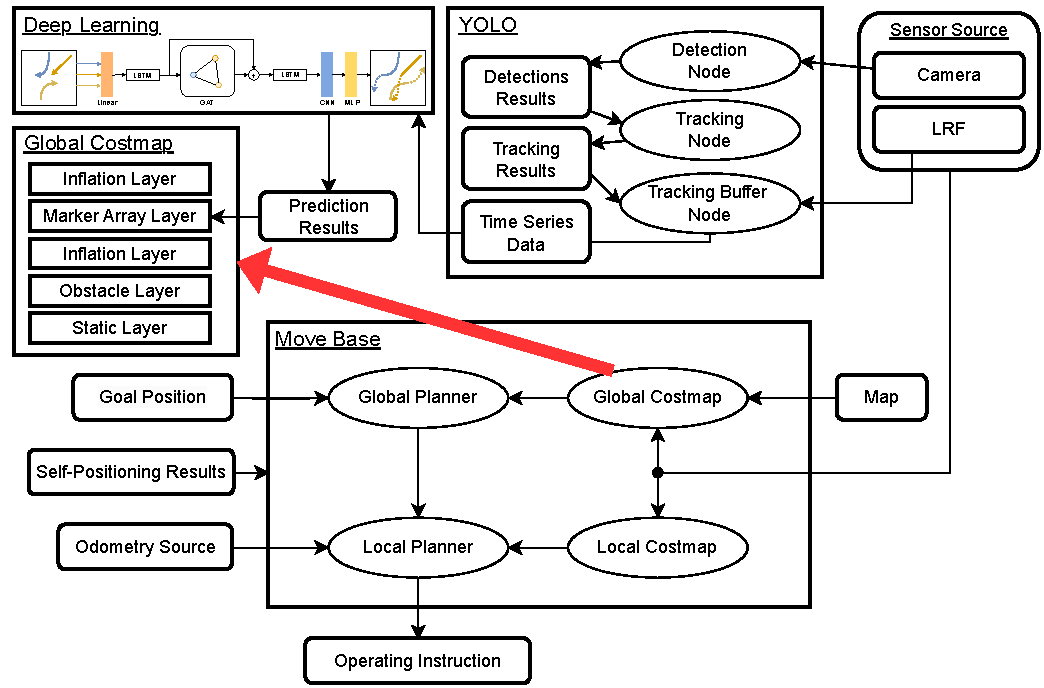
\includegraphics[keepaspectratio, scale=0.77]
      {images/application_system.pdf}
 \caption{Navigation system overview}
 \label{Fig:nav-system}
\end{figure}

\vspace{-30pt}

\section{実ロボットにおける歩行者の位置計算}\label{sec:real-robot}
\figref{Fig:ped2pos}に,俯瞰視点のデータセットと実ロボット上での歩行者の位置計算のイメージを示す.ここで,データセットとはETH\cite{pellegrini2009you-eth}やUCY\cite{lerner2007crowds-ucy}データセットのように,俯瞰視点のデータセットのことを指す.\figref{Fig:ped2pos-dataset}のように,データセットは俯瞰視点の映像と各時刻における歩行者のワールド座標系上の位置が含まれている.しかし,実ロボットで歩行者位置を計算する際は,ロボットがセンサを通じて取得した情報のみを用いてワールド座標系の位置を算出しなければならない.\figref{Fig:ped2pos-realrobot}の例のように,1人称視点で撮影した画像中の歩行者の位置を座標変換することで,ワールド座標系上の位置を得る.これにより,データセットと同じ形式の歩行者の位置データが得られ,データセットで学習したモデルを再学習することなく実ロボット上に適用できる.

\begin{figure}[H]
  \centering
  \begin{minipage}{0.85\textwidth}
    \centering
    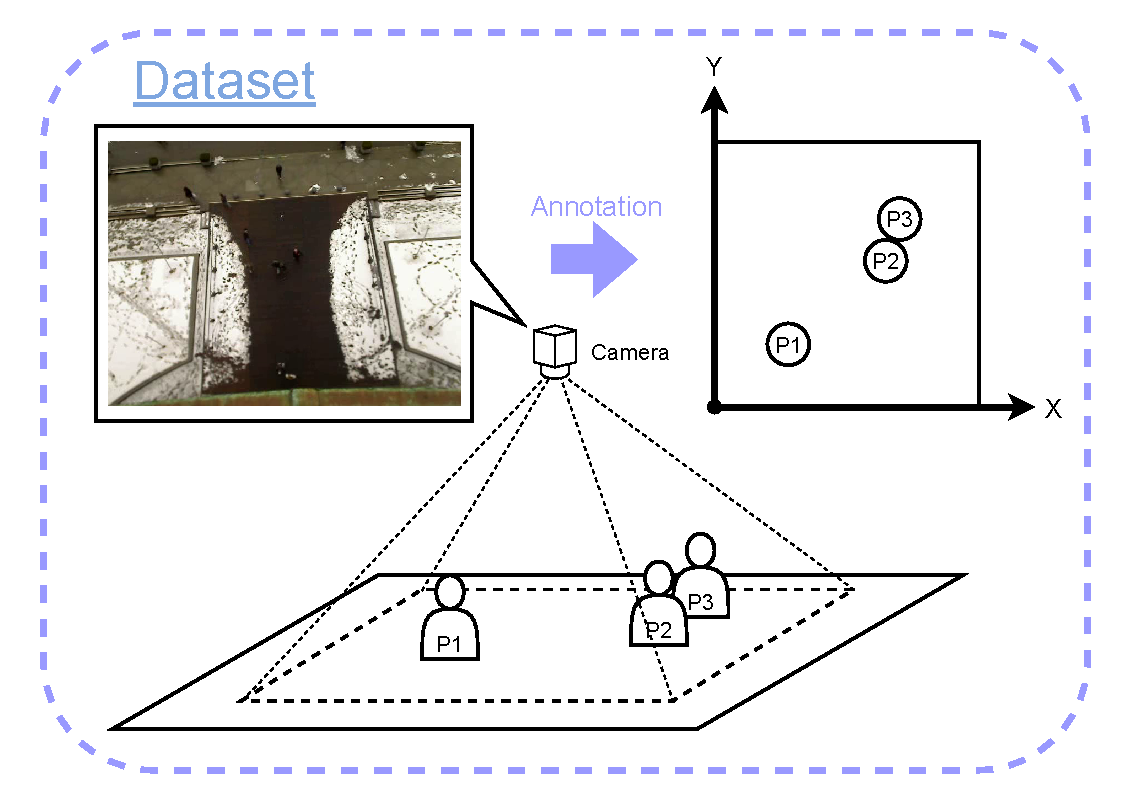
\includegraphics[width=\linewidth]{images/ped2pos-dataset.pdf}
    \subcaption{Pedestrian position calculation on dataset}
    \label{Fig:ped2pos-dataset}
  \end{minipage}
  \hfill
  \begin{minipage}{0.85\textwidth}
    \centering
    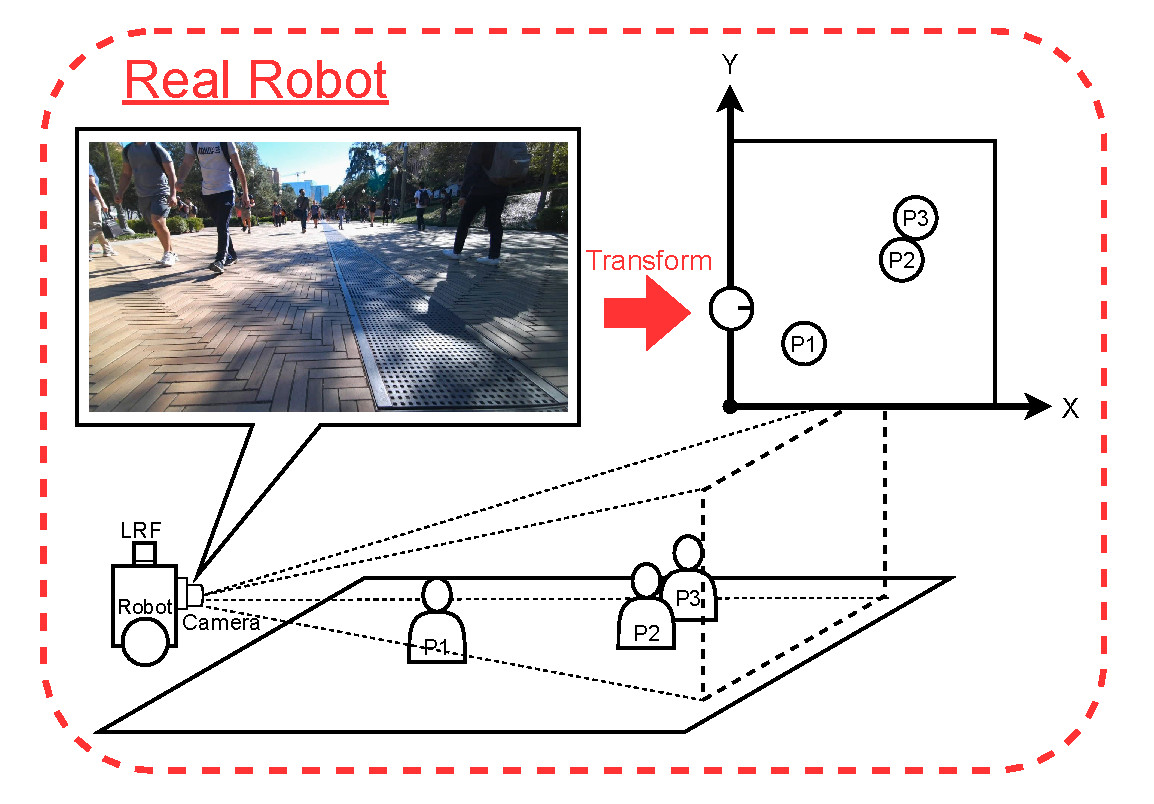
\includegraphics[width=\linewidth]{images/ped2pos-realrobot.pdf}
    \subcaption{Pedestrian position calculation on real robot}
    \label{Fig:ped2pos-realrobot}
  \end{minipage}
  \caption{Pedestrian position calculation: (a) on dataset, (b) on real robot}
  \label{Fig:ped2pos}
\end{figure}
% \protect\footnotetext[8]{\cite{pellegrini2009you-eth}より画像を引用}
% \protect\footnotetext[9]{\cite{karnan2022socially-scand}より画像を引用}

\newpage

本研究での実ロボットにおける歩行者の位置計算の流れと詳細を以下に示す.

\begin{enumerate}
  \item \textbf{RGBカメラ画像とLRFデータを取得} \\
  ロボット前方に取り付けたRGBカメラから歩行者の画像を取得し,同時にLRF(Laser Range Finder)から周囲の距離データを得る.いずれも歩行者の位置計算に必要となる情報を提供する.

  \item \textbf{YOLOで人間検出} \\
  YOLO\cite{redmon2016you-yolo}は,高速・高精度な物体検出アルゴリズムであり,RGBカメラ画像から歩行者を検出する.本研究では,YOLOv9\cite{wang2025yolov9}の学習済みモデル(yolov9c.pt)を使用し,画像上で歩行者の位置を特定する.

  \item \textbf{検出した個体の画像上での角度を計算} \\
  検出した歩行者の画像上での位置をもとに,式\eqref{yolo-ang}に従いロボットカメラの視野内における角度$\theta_{camera}$を求める.
  \begin{equation}
    \theta_{camera} = - \cfrac{(x_{center} - \cfrac{w_{img}}{2}) \cdot fov_{horizontal}}{W_{img}} \label{yolo-ang}
  \end{equation}

  ここで,$w_{img}$は画像の幅,$fov_{horizontal}$はカメラの水平視野角,$x_{center}$が検出バウンディングボックスの中心の$x$座標である.計算後,$\theta_{camera}$を$-\pi \text{から} \pi$の範囲に正規化する.

  \item \textbf{計算した角度とLRFデータからロボットとの相対位置を計算} \\
  画像上で得られた角度情報に対応するLRFデータの要素を取り出す.そして,そのデータを用いて歩行者とロボットとの相対位置を計算する.LRFはロボットからの距離情報を提供し,歩行者の正確な位置を特定するために使用される.

  \item \textbf{相対位置をワールド座標へ座標変換} \\
  最後に,得られた相対位置をワールド座標系に変換する.この座標変換は,ロボットのナビゲーションシステムのmapフレームに基づいて行われる.ワールド座標系での位置が特定されることで,ロボットは歩行者の位置を正確に把握し,適切なナビゲーションを行うことができる.
\end{enumerate}

\section{ナビゲーションにおける予測結果の利用方法}\label{sec:nav-usage}
\figref{Fig:global-costmap}に示すように,グローバルコストマップに独自のレイヤとしてMarker Array Layerを追加した.このレイヤでは,0.4秒ごとに受け取る予測結果をコストマップへ反映する.
\ref{sec:decoder}項で述べたとおり,予測結果のデータ形式はガウス分布を構成する5次元の要素である.本研究では,そのガウス分布からサンプリングした軌道を予測結果としてコストマップに反映する.
\figref{Fig:costmap-flow}のように,各レイヤでの処理を積み重ねて,最終的なグローバルコストマップを生成する.グローバルコストマップを拡張したのは,\ref{sec:navigation-stack}節で述べたように,多くのロボットで使用されているNavigation stackで予測結果を容易に利用できるようにするためである.

\begin{figure}[H]
  \centering
 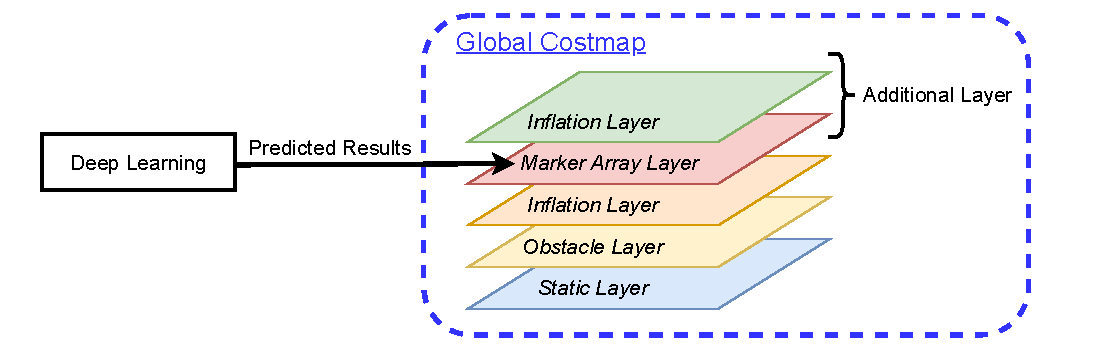
\includegraphics[keepaspectratio, scale=0.65]
      {images/layer.pdf}
\caption{Global costmap with costom layer}
 \label{Fig:global-costmap}
\end{figure} 

\vspace{-20pt}

\begin{figure}[H]
  \centering
 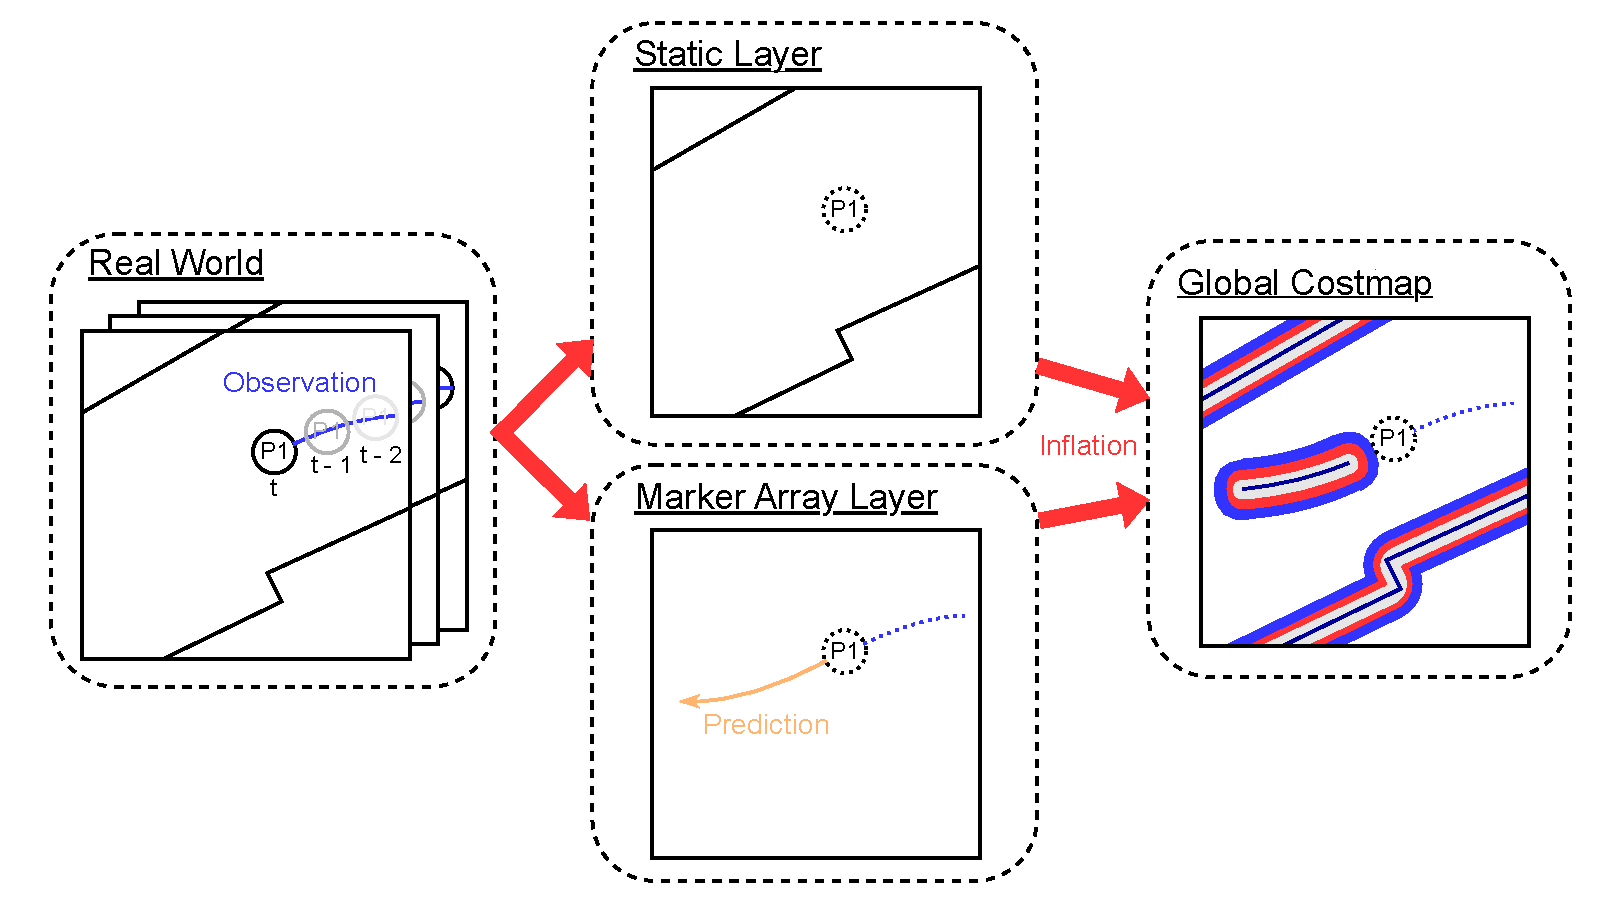
\includegraphics[keepaspectratio, scale=0.45]
      {images/costmap-image.pdf}
\caption{Process each layer to generate a global costmap}
 \label{Fig:costmap-flow}
\end{figure} 


\newpage

%

%ここにディレクトリのパスを追加していく
%
%% Back Matter
\backmatter{}
%
%!TEX root = ../thesis.tex
%\bibliographystyle{plain}
\bibliographystyle{junsrt}
%\bibliography{report}
\nocite{*}
\bibliography{main_bibliography}
%
%!TEX root = ../thesis.tex
\chapter*{付録}
\addcontentsline{toc}{chapter}{付録}

\leftline{\textbf{動画}}

実験の結果から得られたモデルを用いて, 中間層の可視化を行った状態で学習器の出力において走行させた際の動画を記録した. CNNが通路の特徴(輪郭, または壁と床の境界線)を捉えるように学習を行ったことが見て取れる. 以下にアップロードした動画のURLを掲載する.\\
\url{https://youtu.be/JusGVH6ejFg}
%
%!TEX root = ../thesis.tex
\chapter*{謝辞}
\addcontentsline{toc}{chapter}{謝辞}

本研究を進めるにあたり,1年に渡り, 熱心にご指導を頂いた林原靖男教授に深く感謝いたします.ロボット設計制御研究室の皆様には, ご意見, ご協力頂き感謝申し上げます. 特に, 春山健太氏には, 研究の着想や実験など多くの助言をして頂きましたことを心より感謝いたします.
%



%

\end{document}
